% docs/texte/contents.tex -- chapter structure file (Interferosim)
% Version: 0.3.4 (2026-10-12)
% 0.1.0: Kapitelstruktur auf Interferosim umgestellt.
% 0.2.0: Repository structure: chapters grouped in numbered folders
%        (00_frontmatter, 10_engineering, 20_core, 30_notebooks, 40_qa),
%        all titles in English (project language). Part "Software
%        Engineering" (added by E. Schubert) now has its chapters.
% 0.2.1: chapter "Basic Design" (UML diagrams) added.
% 0.3.0: part "Theory" (folder 05_theory) added between front matter
%        and software engineering.
% 0.3.1: "Notation and Conventions" renamed "Notation"; chapters
%        "Conventions" and "Versioning" merged into "Development Guidelines".
% 0.3.2: chapter "Version Control" (git, GitHub) added.
% 0.3.3: chapter "API Documentation" (Doxygen) added.
% 0.3.4: chapter "Data Formats" added.
% ================================================================
\part{Front Matter}

	\chapter{History}
	% docs/texte/00_frontmatter/history.tex -- version history
% (moved from texte/history.tex; 2026-10-12 translated to English)
% ================================================================
% Strukturfile für Kapitel
% ================================================================
\id
% ----------------------------------------------------------------


\index{version history}
Only versions that were officially released are listed here.
Intermediate versions are not listed but can be reconstructed at any
time from version control.


\tabelle{ll l >{\raggedright\arraybackslash}p{8.4cm}}{Version history}{tab:history}{\normalsize}{\hline
    Version & Date & Author & Remark \\
    \hline
    0.0.1 & 2026-10-12 & SE & Initial version, skeleton from uni-work~0.1.1 \\
    0.0.2 & 2026-10-12 & SE & Repository structure, English, project-specific abbreviations \\
    0.0.3 & 2026-10-12 & SE & Basic design: UML package and class diagrams (draft) \\
    0.0.4 & 2026-10-12 & SE & Part \enquote{Theory}; two-element interferometer figure in TikZ \\
    0.0.5 & 2026-10-12 & SE & Appendix with detailed explanations: term \enquote{fringe} \\
    0.0.6 & 2026-10-12 & SE & Chapter \enquote{Development Guidelines}; theory chapter \enquote{Notation} \\
    0.0.7 & 2026-10-12 & SE & Chapter \enquote{Sky Models} (interferosim 0.2.0) \\
    0.0.8 & 2026-10-12 & SE & Project virtual environment; English demo names (interferosim 0.2.1) \\
    0.0.9 & 2026-10-12 & SE & Chapters \enquote{Version Control} and \enquote{Tests and Validation} \\
    0.0.10 & 2026-10-12 & SE & Chapter \enquote{API Documentation} (Doxygen) \\
    0.0.11 & 2026-10-12 & SE & Requirements with IDs, data formats, basic design 0.2 (signal chain, spectra), antenna types \\
    0.0.12 & 2026-10-12 & SE & Known sky regions (A-team, Orion A) with gallery (interferosim 0.2.2) \\
    0.0.13 & 2026-10-12 & SE & Antennas, receiver, chapter \enquote{Stations and Array} (interferosim 0.3.0) \\
    0.0.14 & 2026-10-12 & SE & Choice of the baseline length, example Cyg~A (interferosim 0.3.1) \\
    0.0.15 & 2026-10-31 & SE & B210 device profile, profiles, block diagram of the receive path (interferosim 0.3.2) \\
    0.0.16 & 2026-10-31 & SE & Chapter \enquote{Signal Simulation}, geometry in \enquote{Observation} (interferosim 0.4.0) \\
    0.0.17 & 2026-10-31 & SE & Observation, uv-coverage, visibility and transit simulation, VisData (interferosim 0.5.0) \\
    0.0.18 & 2026-10-31 & SE & Asymmetry of a track; theory notebook A (fringes) (interferosim 0.5.1) \\
    0.0.19 & 2026-10-31 & SE & Chapter \enquote{Correlator} (FX correlator, fringe search) (interferosim 0.6.0) \\
    0.0.20 & 2026-10-31 & SE & Chapter \enquote{Imaging} (gridding, weighting, dirty image) (interferosim 0.7.0) \\
    0.0.21 & 2026-10-31 & SE & Chapter \enquote{Deconvolution} (CLEAN, clean beam, Wiener filter) (interferosim 0.8.0) \\
    0.0.22 & 2026-10-31 & SE & The Sun as the first target (solar transit, radio diameter) (interferosim 0.8.1) \\
    0.0.23 & 2026-11-01 & SE & Chapter \enquote{Spectral Lines} (spectra, LSR correction, channel maps) (interferosim 0.9.0) \\
}


	\chapter{Project Description}
	% docs/texte/00_frontmatter/project.tex -- chapter "Project Description" (Interferosim)
% Version: 0.1.0 (2026-10-12)
% ================================================================

Interferosim is an open-source Python package for simulating radio
interferometers, from a two-element system up to small arrays. It is
developed as a project of the University of Vienna. Scope, target
audience and schedule are defined in the separate project description
(\texttt{docs/projektbeschreibung.tex}).

The software starts from the simulation package \texttt{aas6sim}
(version~1.1.0) of the Antares Astro Software and from two teaching
notebooks (Appendix~A: Wiener filter and CLEAN; Appendix~B: the Sun as
a first target). Their functions are moved into the package; the
notebooks then only call the package.


	\chapter{System Environment}
	% docs/texte/00_frontmatter/environment.tex -- chapter "System Environment" (Interferosim)
% Version: 0.2.0 (2026-10-12) -- project virtual environment
%   0.1.0: placeholder
% ================================================================

Python~$\geq$~3.11 with numpy, scipy, matplotlib and astropy; JupyterLab,
ipywidgets and ipykernel for the notebooks; pytest and nbval for the
tests. The notebooks run locally, on JupyterHub or on Binder
(\texttt{binder/environment.yml}).

\section{Project virtual environment}
\index{virtual environment}

All work uses the virtual environment \texttt{.venv} in the project
folder (excluded from version control by \texttt{.gitignore}). It is
created by a script:

\begin{center}
\begin{tabular}{@{}ll@{}}
\toprule
System & Command (in the project folder) \\
\midrule
Windows & \texttt{setup\_venv.bat} (double-click) or\\
        & \texttt{powershell -ExecutionPolicy Bypass -File setup\_venv.ps1} \\
Linux, macOS & \texttt{./setup\_venv.sh} \\
\bottomrule
\end{tabular}
\end{center}

The script searches for Python~$\geq$~3.11, creates \texttt{.venv}, installs
Interferosim in editable mode with the extras \texttt{notebooks} and
\texttt{test}, registers the Jupyter kernel \enquote{Python
(interferosim)} and runs the tests. Options of the Windows script:
\texttt{-Python <path>} (explicit interpreter), \texttt{-Recreate}
(delete and rebuild \texttt{.venv}), \texttt{-NoTests},
\texttt{-DropboxIgnore} (exclude \texttt{.venv} from Dropbox
synchronisation).

After activation (\texttt{.venv\textbackslash Scripts\textbackslash activate}
on Windows, \texttt{source .venv/bin/activate} on Linux/macOS) the command
line tool \texttt{interferosim-sky} and \texttt{jupyter lab} are available.


\part{Theory}

	\chapter{Notation}
	% docs/texte/05_theory/notation.tex -- theory chapter "Notation" (Interferosim)
% Version: 0.1.1 (2026-10-12)
% 0.1.1: chapter renamed "Notation and Conventions" -> "Notation";
%        paragraph "Conventions" -> "General assumptions" (no confusion with
%        the coding conventions in part "Software Engineering")
% Notation as defined in texte/05_theory/notation.tex.
% ================================================================

\index{notation}
This part collects the physical and mathematical basis of
Interferosim. All chapters use the notation of
Table~\ref{tab:notation}; the same symbols are used in the code
documentation and in the notebooks. Standard references are
\cite{thompson2017,condon2016,wilson2013,taylor1999}.

\paragraph*{General assumptions.}
\begin{itemize}
  \item SI units throughout; flux densities in jansky,
        $1\,\mathrm{Jy} = 10^{-26}\,\mathrm{W\,m^{-2}\,Hz^{-1}}$;
        solar flux unit $1\,\mathrm{SFU} = 10^{4}\,\mathrm{Jy}$.
  \item Spatial frequencies $u,v,w$ are measured in \emph{wavelengths},
        baselines $\vec b$ in metres.
  \item Sky coordinates $(l,m)$ are direction cosines relative to the
        phase centre; for small fields they equal angular offsets in
        radians.
  \item The Fourier sign convention is $V = \int I\,e^{-2\pi i(ul+vm)}$
        (sky $\to$ visibility) and $I = \int V\,e^{+2\pi i(ul+vm)}$
        (visibility $\to$ sky).
  \item Brightness temperatures use the Rayleigh--Jeans approximation
        ($h\nu \ll kT$). At 1.4\,GHz, $h\nu/k \approx 0.07\,\mathrm{K}$;
        the relative error $\approx h\nu/2kT$ is below $10^{-3}$ for
        $T > 35\,\mathrm{K}$, which holds for all sources considered.
\end{itemize}

\begin{longtable}{@{}>{$}l<{$}l>{\raggedright\arraybackslash}p{8.2cm}@{}}
\caption{Symbols used in this documentation}\label{tab:notation}\\
\toprule
\textrm{Symbol} & Unit & Meaning \\
\midrule
\endfirsthead
\toprule
\textrm{Symbol} & Unit & Meaning \\
\midrule
\endhead
\bottomrule
\endfoot
\multicolumn{3}{@{}l}{\textit{Constants}}\\
c & m\,s$^{-1}$ & speed of light, $299\,792\,458$ \\
k & J\,K$^{-1}$ & Boltzmann constant, $1.380649\times10^{-23}$ \\
\omega_E & rad\,s$^{-1}$ & Earth rotation rate, sidereal
  $7.292115\times10^{-5}$; for the Sun $\omega_\odot = 2\pi/86\,400\,\mathrm{s}$ \\
\multicolumn{3}{@{}l}{\textit{Radiation and source}}\\
\nu,\ \lambda & Hz, m & observing frequency and wavelength, $\lambda = c/\nu$ \\
\Delta\nu & Hz & bandwidth \\
I(l,m) & Jy\,sr$^{-1}$ & sky brightness (specific intensity) \\
T_b & K & brightness temperature \\
S & Jy & flux density \\
\Omega & sr & solid angle (of a source) \\
\theta_d & rad & diameter of a uniform disc \\
\theta_{1/2} & rad & FWHM of a Gaussian source \\
\multicolumn{3}{@{}l}{\textit{Antenna and receiver}}\\
D & m & dish diameter \\
\eta_A & -- & aperture efficiency \\
A_{\mathrm{eff}} & m$^2$ & effective area \\
G & -- & gain (often quoted in dBi) \\
\theta_{\mathrm{HPBW}} & rad & half-power beam width \\
k_b & -- & beam factor, $\theta_{\mathrm{HPBW}} = k_b\,\lambda/D$ \\
A(l,m) & -- & normalised primary beam \\
T_A,\ T_{\mathrm{sys}} & K & antenna and system temperature \\
\mathrm{SEFD} & Jy & system equivalent flux density \\
\tau & s & integration time \\
\rho & -- & correlation coefficient \\
\multicolumn{3}{@{}l}{\textit{Geometry}}\\
\vec b,\ b & m & baseline vector and length \\
L_X, L_Y, L_Z & m & baseline components in equatorial coordinates \\
\hat s & -- & unit vector towards the source \\
\tau_g & s & geometric delay, $\tau_g = \vec b\cdot\hat s/c$ \\
\theta & rad & angle between baseline and source direction \\
H,\ \delta & rad & hour angle and declination of the source \\
\varphi & rad & geographic latitude of the site \\
\varepsilon & rad & elevation \\
\multicolumn{3}{@{}l}{\textit{Fourier domain and imaging}}\\
u,v,w & $\lambda$ & spatial frequencies (baseline in wavelengths) \\
q & $\lambda$ & radial spatial frequency, $q = \sqrt{u^2+v^2}$ \\
l,m & -- & direction cosines \\
\mathcal{V}(u,v) & Jy & complex visibility \\
\mathcal{S}(u,v) & -- & sampling (transfer) function \\
W(u,v) & -- & imaging weights \\
I_D,\ B_D & Jy\,beam$^{-1}$, -- & dirty image, dirty beam \\
B_C & -- & clean beam \\
\mathcal{W} & -- & Wiener filter \\
\Phi_s,\ \Phi_n & -- & power spectra of signal and noise \\
f_F & Hz & fringe frequency (fringe rate) \\
\end{longtable}


	\chapter{Radio Astronomical Fundamentals}
	% docs/texte/05_theory/fundamentals.tex -- theory chapter "Radio Astronomical Fundamentals" (Interferosim)
% Version: 0.1.0 (2026-10-12)
% Notation as defined in texte/05_theory/notation.tex.
% ================================================================

\index{brightness temperature}\index{antenna temperature}
\section{Brightness temperature and flux density}

In the Rayleigh--Jeans limit the specific intensity of a black body is
\begin{equation}
  I_\nu = \frac{2\,k\,T_b}{\lambda^2} .
\end{equation}
The brightness temperature $T_b$ is defined by this relation for any
source, thermal or not. The flux density is the intensity integrated
over the source,
\begin{equation}
  S = \int_{\mathrm{source}} I_\nu\,\mathrm{d}\Omega
    \;\approx\; \frac{2\,k\,T_b\,\Omega}{\lambda^2}
  \qquad\text{(uniform source).}
  \label{eq:flux-tb}
\end{equation}
\emph{Example (notebook~B):} the quiet Sun at 21\,cm has
$T_b \approx 10^5\,\mathrm{K}$ and a radio diameter of about $34'$, which
gives $S \approx 4.8\times10^5\,\mathrm{Jy} \approx 48\,\mathrm{SFU}$.
Both quantities vary with the solar cycle by about a factor of two.

\section{Antennas}

An antenna collects power from a solid angle given by its beam. The
effective area $A_{\mathrm{eff}}$ and the gain $G$ are related by
\begin{equation}
  G = \frac{4\pi A_{\mathrm{eff}}}{\lambda^2}.
  \label{eq:gain-area}
\end{equation}
For a parabolic dish $A_{\mathrm{eff}} = \eta_A\,\pi D^2/4$; the
half-power beam width is
\begin{equation}
  \theta_{\mathrm{HPBW}} = k_b\,\frac{\lambda}{D},
\end{equation}
with $k_b = 1.02$ for uniform illumination and $k_b \approx 1.2$ for a
typical tapered feed (used in the simulations). For an antenna specified
only by its gain (e.\,g.\ a horn), the beam solid angle is
$\Omega_A = 4\pi/G$; with a Gaussian main beam,
$\Omega_A = 1.133\,\theta_{\mathrm{HPBW}}^2$, so
\begin{equation}
  \theta_{\mathrm{HPBW}} = \sqrt{\frac{4\pi}{1.133\,G}} .
\end{equation}

\paragraph*{Antenna temperature.} A source of flux density $S$ raises
the antenna temperature by
\begin{equation}
  T_A = \frac{A_{\mathrm{eff}}\,S}{2k},
  \label{eq:ta}
\end{equation}
where the factor $1/2$ accounts for a single polarisation receiving an
unpolarised source. For a source larger than the beam only the part
inside the beam contributes.

\section{Sensitivity}

The receiver adds noise of temperature $T_{\mathrm{sys}}$. Expressed as
the flux density that would produce the same antenna temperature,
\begin{equation}
  \mathrm{SEFD} = \frac{2\,k\,T_{\mathrm{sys}}}{A_{\mathrm{eff}}} .
\end{equation}
The radiometer equation gives the noise of a total-power measurement
with bandwidth $\Delta\nu$ and integration time $\tau$:
\begin{equation}
  \sigma_T = \frac{T_{\mathrm{sys}}}{\sqrt{\Delta\nu\,\tau}} .
  \label{eq:radiometer}
\end{equation}
A strong source raises the total noise: if $T_A$ is not small compared
with $T_{\mathrm{sys}}$, $T_{\mathrm{sys}}$ must be replaced by
$T_{\mathrm{sys}} + T_A$. For the Sun observed with a 3\,m dish
($T_A \approx 730\,\mathrm{K}$ against $T_{\mathrm{sys}} = 120\,\mathrm{K}$)
the receiver must also stay linear, which requires an attenuator in
front of the LNA.

\section{Spectral lines}

Interferosim supports the following lines (rest frequencies, see
\texttt{interferosim.constants}):
\begin{center}
\begin{tabular}{@{}lll@{}}
\toprule
Line & Frequency [MHz] & Remark \\
\midrule
HI 21\,cm & 1420.405\,751\,768 & hyperfine transition of neutral hydrogen \\
OH & 1612.231 & satellite line \\
OH & 1665.402 & main line \\
OH & 1667.359 & main line \\
OH & 1720.530 & satellite line \\
\bottomrule
\end{tabular}
\end{center}


	\chapter{The Two-Element Interferometer}
	% docs/texte/05_theory/two_element.tex -- theory chapter "The Two-Element Interferometer" (Interferosim)
% Version: 0.1.1 (2026-10-12) -- figure source note, reference to appendix
% Notation as defined in texte/05_theory/notation.tex.
% ================================================================

\index{interferometer!two-element}\index{geometric delay}
\section{Geometric delay and fringes}

Figure~\ref{fig:two-element} shows two antennas separated by the
baseline $\vec b$. A plane wave from the direction $\hat s$ reaches
antenna~1 later than antenna~2 by the \emph{geometric delay}
\begin{equation}
  \tau_g = \frac{\vec b\cdot\hat s}{c} = \frac{b\cos\theta}{c} .
  \label{eq:taug}
\end{equation}
For a monochromatic signal the voltages are
$V_1 = V\cos[\omega(t-\tau_g)]$ and $V_2 = V\cos(\omega t)$. A
multiplying correlator forms $V_1V_2$ and averages over a time long
compared with $1/\omega$:
\begin{equation}
  R = \langle V_1 V_2\rangle = \frac{V^2}{2}\cos(\omega\tau_g) .
  \label{eq:fringe}
\end{equation}
As the source direction changes, $R$ oscillates: these are the
\emph{fringes}. Their angular spacing near $\theta = 90^\circ$ is
$\lambda/b$; this is the angular resolution scale of the baseline.
Appendix~\ref{app:fringe} explains the term \enquote{fringe} and the
related terms in detail.

\begin{figure}[htbp]
  \centering
  % docs/texte/05_theory/figures/two_element_interferometer.tex -- two-element interferometer (TikZ)
% Version: 0.1.1 (2026-10-12) -- signal labels below the lines (no overlap with 12 pt text)
% Redrawn in TikZ after docs/images/antennengeometrie2.png (two-element
% interferometer with multiplying correlator). Geometry: baseline b along
% the x axis, source direction s at angle theta to the baseline; the
% wavefront through antenna 2 meets the line from antenna 1 along s at P,
% so |0P| = b cos(theta) = c tau_g.
\begin{tikzpicture}[>=Stealth, font=\footnotesize]
  % ---- parameters ---------------------------------------------------
  \def\b{6.0}        % baseline length (drawing units)
  \def\th{55}        % angle theta between baseline and source direction
  \pgfmathsetmacro{\px}{\b*cos(\th)*cos(\th)}
  \pgfmathsetmacro{\py}{\b*cos(\th)*sin(\th)}
  \coordinate (A1) at (0,0);
  \coordinate (A2) at (\b,0);
  \coordinate (P)  at (\px,\py);

  % ---- source direction and wavefront ------------------------------
  \draw[thin] (A1) -- (P);
  \draw[thin,dotted] (P) -- ($(A1)!1.75!(P)$);
  \draw[->,thick] ($(A1)!1.75!(P)$) -- ($(A1)!1.95!(P)$)
        node[above right=-1pt] {$\hat{s}$};
  \draw[thin,dotted] (A2) -- ++(\th:3.6);
  \draw[thin] (A2) -- (P);                                   % wavefront
  \draw[thin] (A1) -- node[below=3pt] {$\vec{b}$} (A2);       % baseline
  % path difference along s
  \path (A1) -- (P) node[midway,sloped,above=2pt]
        {$c\,\tau_g = \vec{b}\cdot\hat{s}$};
  % angle theta
  \draw (1.5,0) arc[start angle=0,end angle=\th,radius=1.5];
  \node at ({\th/2}:1.8) {$\theta$};
  % right angle at P
  \draw[thin] ($(P)!0.22cm!(A1)$) -- ++(\th-90:0.22cm) -- ($(P)!0.22cm!(A2)$);

  % ---- antennas: reflector arc on a mount (triangle) ---------------
  \foreach \A/\n in {A1/1, A2/2}{
    \draw[very thick] ($(\A)+(-1.1,0.55)$) .. controls ($(\A)+(-0.45,-0.05)$)
          and ($(\A)+(0.45,-0.05)$) .. ($(\A)+(1.1,0.55)$);
    \draw[thick] (\A) -- ++(-0.38,-1.25) -- ++(0.76,0) -- cycle;
    \node at ($(\A)+(0,-0.85)$) {\n};
  }

  % ---- signal path: multiplier and averaging -----------------------
  \coordinate (M) at ({\b/2},-2.4);
  \draw[thick] (A1) ++(0,-1.25) |- ($(M)+(-0.32,0)$);
  \draw[thick] (A2) ++(0,-1.25) |- ($(M)+(0.32,0)$);
  \draw[thick] (M) circle[radius=0.32];
  \draw[thick] (M) ++(-0.2,-0.2) -- ++(0.4,0.4) (M) ++(-0.2,0.2) -- ++(0.4,-0.4);
  \node[anchor=north east] at ($(M)+(-0.4,-0.08)$) {$V_1 = V\cos[\omega(t-\tau_g)]$};
  \node[anchor=north west] at ($(M)+(0.4,-0.08)$)  {$V_2 = V\cos(\omega t)$};
  \node[draw,thick,minimum width=1.1cm,minimum height=0.55cm] (avg)
        at ($(M)+(0,-2.1)$) {$\langle\;\rangle$};
  \draw[thick] ($(M)+(0,-0.32)$) -- node[right,pos=0.6] {$V_1V_2$} (avg.north);

  % ---- correlator output: fringe pattern ----------------------------
  \draw[->,thick] (avg.east) -- ++(0.5,0);
  \draw[thin,domain=0:6,samples=400,smooth]
     plot ({\b/2+1.25+\x},{-4.5+0.42*exp(-((\x-3)^2)/1.8)*cos(deg(9.5*\x))});
  \node at ({\b/2+4.25},-5.2) {$R = \tfrac{V^2}{2}\cos(\omega\tau_g)$};
\end{tikzpicture}

  \caption{Two-element interferometer with multiplying correlator. Both
           antennas receive the same signal, delayed by
           $\tau_g = \vec b\cdot\hat s/c$; the averaged product depends
           on the source direction through $\tau_g$. Redrawn after a
           schematic that appears in many publications without a
           traceable original, e.\,g.\ \cite{krinkele2012}.}
  \label{fig:two-element}
\end{figure}
\addtocategory{pic}{krinkele2012}  % listed under figure sources

\section{Complex correlator}

The cosine correlator of Eq.~\eqref{eq:fringe} responds only to the
even part of the brightness distribution. A second correlator with a
$90^\circ$ phase shift in one signal path gives the sine component. Both
together form the \emph{complex visibility} (chapter~\ref{ch:visibility}).
With an SDR receiver both signals are available as complex IQ samples,
so the complex product $x_1 x_2^*$ yields both components directly.

\section{Fringe rate}

The Earth's rotation changes $\tau_g$ continuously. For an east--west
baseline of length $b$ the delay and the fringe frequency are
\begin{equation}
  \tau_g = \frac{b}{c}\cos\delta\,\sin H , \qquad
  f_F = \frac{b}{\lambda}\,\cos\delta\,\cos H\;\omega_E .
  \label{eq:fringerate}
\end{equation}
The fringe rate is largest at transit ($H=0$). For the Sun the solar
rate $\omega_\odot$ must be used instead of the sidereal rate
$\omega_E$; the difference of 0.27\,\% shifts each fringe of a
5-minute period by almost one second.

\section{Bandwidth and delay}

With a finite bandwidth $\Delta\nu$ the fringes of different
frequencies add with different phases. For a rectangular passband the
fringe amplitude is reduced by
\begin{equation}
  \left|\operatorname{sinc}(\Delta\nu\,\tau)\right|, \qquad
  \operatorname{sinc}x = \frac{\sin\pi x}{\pi x},
\end{equation}
where $\tau$ is the residual delay after compensation. Without delay
compensation $\tau = \tau_g$; this limits uncompensated operation to
short baselines (for $\Delta\nu = 2\,\mathrm{MHz}$: loss below 1\,\% up
to $b \approx 10\,\mathrm{m}$). Long baselines need delay tracking.

\section{Sensitivity of an interferometer}

For two antennas observing a point source the correlation coefficient
is
\begin{equation}
  \rho = \frac{\sqrt{T_{A,1}\,T_{A,2}}}
              {\sqrt{(T_{\mathrm{sys},1}+T_{A,1})(T_{\mathrm{sys},2}+T_{A,2})}}
  \;\xrightarrow{\text{identical}}\;
  \frac{T_A}{T_{\mathrm{sys}}+T_A}.
\end{equation}
For a resolved source $\rho$ is multiplied by the normalised
visibility $|\mathcal V|/S$. With Nyquist-sampled signals of bandwidth
$\Delta\nu$ a correlator averages $N = 2\Delta\nu\tau$ independent
products; the noise of each correlator output is $1/\sqrt{N}$ in units
of $\rho$, so
\begin{equation}
  \mathrm{SNR} = \rho\,\sqrt{2\,\Delta\nu\,\tau} .
  \label{eq:snr-corr}
\end{equation}

\section{Adding and multiplying interferometer}

An \emph{adding} interferometer sums the two signals and measures the
total power with a detector. The output is the total-power level plus
the fringe term; the peak-to-peak fringe amplitude relative to the total
power is $2\rho\,|\mathcal V|/S$. A total-power detector is therefore
usable only if the receiver gain is stable to a fraction of this value.
A \emph{multiplying} interferometer outputs only the correlated part and
is insensitive to gain drifts of the uncorrelated noise. Interferosim
models both in \texttt{observation.Correlator}.


	\chapter{Visibility and Source Models}
	% docs/texte/05_theory/visibility.tex -- theory chapter "Visibility and Source Models" (Interferosim)
% Version: 0.1.0 (2026-10-12)
% Notation as defined in texte/05_theory/notation.tex.
% ================================================================

\label{ch:visibility}
\index{visibility}\index{van Cittert--Zernike theorem}
\section{The visibility function}

For a field small enough that the $w$ term can be neglected, the
response of a baseline $(u,v)$ to the brightness distribution $I(l,m)$
is the complex visibility
\begin{equation}
  \mathcal V(u,v) = \iint A(l,m)\,I(l,m)\,
     e^{-2\pi i\,(ul+vm)}\,\mathrm{d}l\,\mathrm{d}m .
  \label{eq:vis}
\end{equation}
This is the van Cittert--Zernike theorem: the visibility is the
two-dimensional Fourier transform of the sky brightness weighted by
the primary beam $A(l,m)$. Since $I$ is real,
$\mathcal V(-u,-v) = \mathcal V^*(u,v)$; every baseline therefore
measures two points of the $(u,v)$ plane.

\section{Analytic visibilities}

Interferosim computes the visibilities of its source components
analytically (\texttt{SkyComponent.visibility}). With $q=\sqrt{u^2+v^2}$:

\paragraph*{Point source} of flux density $S$ at $(l_0,m_0)$:
\begin{equation}
  \mathcal V = S\,e^{-2\pi i\,(ul_0+vm_0)} .
\end{equation}

\paragraph*{Gaussian source} with FWHM $\theta_{1/2}$ (circular):
\begin{equation}
  \mathcal V = S\,\exp\!\left(-\frac{\pi^2\,\theta_{1/2}^2\,q^2}{4\ln 2}\right)
  e^{-2\pi i\,(ul_0+vm_0)} .
\end{equation}
For an elliptical source, $\theta_{1/2}^2 q^2$ is replaced by
$\theta_{\mathrm{maj}}^2 u'^2 + \theta_{\mathrm{min}}^2 v'^2$ with
$(u',v')$ rotated by the position angle.

\paragraph*{Uniform disc} of diameter $\theta_d$:
\begin{equation}
  \mathcal V = S\,\frac{2J_1(\pi\theta_d q)}{\pi\theta_d q} .
  \label{eq:vis-disc}
\end{equation}
The first zero lies at $\pi\theta_d q = 3.8317$, i.\,e.\ at
\begin{equation}
  b_{\mathrm{null}} = 1.2197\,\frac{\lambda}{\theta_d} .
\end{equation}
For the Sun at 21\,cm ($\theta_d = 34'$) this is $b_{\mathrm{null}}
\approx 26\,\mathrm{m}$; measuring the position of the null is a
measurement of the radio diameter (notebook~B).

\paragraph*{Circularly symmetric source} with radial profile $I(r)$,
e.\,g.\ a limb-brightened solar disc: the two-dimensional Fourier
transform reduces to a Hankel transform,
\begin{equation}
  \mathcal V(q) = 2\pi\int_0^{R} I(r)\,J_0(2\pi q r)\,r\,\mathrm{d}r .
\end{equation}
Fitting the uniform-disc model \eqref{eq:vis-disc} to data of a
limb-brightened disc biases the diameter: the formal fit error then
underestimates the true error by a large factor, because the model, not
the noise, dominates the error budget.


	\chapter{Earth Rotation Synthesis and uv-Coverage}
	% docs/texte/05_theory/uv_coverage.tex -- theory chapter "Earth Rotation Synthesis and uv-Coverage" (Interferosim)
% Version: 0.1.0 (2026-10-12)
% Notation as defined in texte/05_theory/notation.tex.
% ================================================================

\index{uv-coverage}\index{Earth rotation synthesis}
\section{Baseline coordinates}

Baselines are expressed in an equatorial system: $X$ towards
$(H=0,\delta=0)$, $Y$ towards $(H=-6^{\mathrm h},\delta=0)$ (east) and
$Z$ towards the celestial pole. A baseline given in local coordinates
(east $E$, north $N$, up $U$) at latitude $\varphi$ becomes
\begin{equation}
  L_X = -N\sin\varphi + U\cos\varphi,\qquad
  L_Y = E,\qquad
  L_Z = N\cos\varphi + U\sin\varphi .
\end{equation}

\section{Spatial frequencies}

For a source at hour angle $H$ and declination $\delta$:
\begin{equation}
  \begin{pmatrix} u\\ v\\ w \end{pmatrix}
  = \frac{1}{\lambda}
  \begin{pmatrix}
    \sin H & \cos H & 0\\
    -\sin\delta\cos H & \sin\delta\sin H & \cos\delta\\
    \cos\delta\cos H & -\cos\delta\sin H & \sin\delta
  \end{pmatrix}
  \begin{pmatrix} L_X\\ L_Y\\ L_Z \end{pmatrix} .
  \label{eq:uvw}
\end{equation}
For an east--west baseline ($L_X=L_Z=0$, $L_Y=b$) this gives
\begin{equation}
  u = \frac{b}{\lambda}\cos H,\qquad
  v = \frac{b}{\lambda}\sin\delta\,\sin H .
\end{equation}

\section{Earth rotation synthesis}

As $H$ changes, each baseline traces an ellipse in the $(u,v)$ plane,
\begin{equation}
  u^2 + \left(\frac{v - (L_Z/\lambda)\cos\delta}{\sin\delta}\right)^2
  = \frac{L_X^2+L_Y^2}{\lambda^2},
\end{equation}
together with its Hermitian mirror image. The axis ratio is
$\sin\delta$; a source near the equator gives a strongly flattened track.
The usable hour-angle range is limited by the elevation of the source,
\begin{equation}
  \sin\varepsilon = \sin\varphi\sin\delta + \cos\varphi\cos\delta\cos H ,
\end{equation}
and a minimum elevation (Interferosim:
\texttt{Observation.min\_elev\_deg}).

\section{Coverage and image quality}

The set of measured $(u,v)$ points defines the sampling function
$\mathcal S(u,v)$. The longest projected baseline sets the resolution,
$\theta \approx \lambda/b_{\max}$; the shortest one sets the largest
angular scale that can be recovered, $\approx\lambda/b_{\min}$.
Emission on larger scales is filtered out. With a single baseline the
coverage is one ellipse; for the 11.5\,km example baseline less than
0.1\,\% of the cells of a typical image grid are occupied
(notebook~A).


	\chapter{Imaging}
	% docs/texte/05_theory/imaging.tex -- theory chapter "Imaging" (Interferosim)
% Version: 0.1.0 (2026-10-12)
% Notation as defined in texte/05_theory/notation.tex.
% ================================================================

\index{dirty image}\index{dirty beam}\index{weighting}
\section{Dirty image and dirty beam}

The measured visibilities are $\mathcal S(u,v)\,\mathcal V(u,v)$. Their
inverse Fourier transform, with imaging weights $W(u,v)$, is the
\emph{dirty image}
\begin{equation}
  I_D(l,m) = \iint W\,\mathcal S\,\mathcal V\;
             e^{+2\pi i\,(ul+vm)}\,\mathrm{d}u\,\mathrm{d}v
           = (A\,I) * B_D ,
\end{equation}
the true (beam-weighted) sky convolved with the \emph{dirty beam}
\begin{equation}
  B_D(l,m) = \iint W\,\mathcal S\;e^{+2\pi i\,(ul+vm)}\,\mathrm{d}u\,\mathrm{d}v .
\end{equation}
$B_D$ is the point spread function (PSF) of the array. Normalising
$B_D(0,0)=1$ gives $I_D$ in Jy\,beam$^{-1}$: a point source shows its
flux density as peak value.

\section{Gridding}

To use the FFT, the visibilities are placed on a regular grid of
$N\times N$ cells. For an image of $N$ pixels of size $\Delta l$ the
cell size in the $(u,v)$ plane is $\Delta u = 1/(N\,\Delta l)$.
Interferosim currently uses nearest-cell gridding (each sample is added
to the nearest cell); convolutional gridding is a possible extension.

\section{Weighting}

The weights $W$ trade sensitivity against beam shape:
\begin{itemize}
  \item \textbf{Natural weighting}: every sample has the same weight
        (or $1/\sigma^2$). Best signal-to-noise ratio, but densely
        sampled regions dominate and the beam has higher sidelobes.
  \item \textbf{Uniform weighting}: every occupied cell has the same
        weight, $W_k = 1/N_k$ for $N_k$ samples in cell $k$. Better
        beam, more noise.
  \item \textbf{Robust (Briggs) weighting} \cite{briggs1995}
        interpolates continuously between both.
\end{itemize}
The Wiener weighting of chapter~\ref{ch:deconvolution} is another
interpolation of the same kind.


	\chapter{Deconvolution}
	% docs/texte/05_theory/deconvolution.tex -- theory chapter "Deconvolution" (Interferosim)
% Version: 0.1.0 (2026-10-12)
% Notation as defined in texte/05_theory/notation.tex.
% ================================================================

\label{ch:deconvolution}
\index{deconvolution}\index{CLEAN}\index{Wiener filter}
Deconvolution estimates the true sky from the dirty image. Two
methods are implemented; which one is suitable depends on whether the
transfer function $\mathcal S$ has zeros.

\section{Wiener filter}

In the Fourier domain the measurement is
\begin{equation}
  D(u,v) = \mathcal S(u,v)\,\tilde I(u,v) + N(u,v)
\end{equation}
with the true image $\tilde I$, the transfer function $\mathcal S$ and
noise $N$. The linear filter $\mathcal W$ that minimises the mean square
error $E|\hat I - I|^2$ of $\hat I = \mathcal W D$ is the Wiener filter
\cite{wiener1949}
\begin{equation}
  \mathcal W = \frac{\mathcal S^*}{|\mathcal S|^2 + \Phi_n/\Phi_s}
  \label{eq:wiener}
\end{equation}
with the power spectra $\Phi_s$ of the signal and $\Phi_n$ of the
noise. For $\Phi_n\to0$ it becomes the inverse filter $1/\mathcal S$;
where the noise dominates it suppresses instead of amplifying.

\paragraph*{Filled aperture.} For a single dish of diameter $D$ the
transfer function is the autocorrelation of the circular aperture,
\begin{equation}
  \mathcal S(q) = \frac{2}{\pi}\left[\arccos\frac{q}{q_c}
     - \frac{q}{q_c}\sqrt{1-\frac{q^2}{q_c^2}}\right],
  \qquad q_c = \frac{D}{\lambda},
\end{equation}
non-zero everywhere below $q_c$. The Wiener filter compensates its
decrease and recovers resolution up to the diffraction limit
(\texttt{deconvolution.WienerFilter}).

\paragraph*{Sparse sampling.} Where $\mathcal S = 0$, Eq.~\eqref{eq:wiener}
gives $\mathcal W D = 0$ exactly. No linear filter can fill unmeasured
cells. For an interferometer, where $\mathcal S$ is either zero or the
number of samples $N_k$ of a cell, the filter reduces to
$\mathcal W_k = N_k/(N_k^2+K)$ with $K=\Phi_n/\Phi_s$: natural
weighting for $K\gg N_k^2$, uniform weighting for $K\ll N_k^2$. It is
therefore modelled as \texttt{imaging.WienerWeighting}.

\section{Högbom CLEAN}

CLEAN \cite{hogbom1974} assumes that the sky consists of a limited
number of point sources:
\begin{enumerate}
  \item Find the peak of the residual image (initially $I_D$).
  \item Subtract the dirty beam, shifted to the peak position and
        scaled by the loop gain $g$ (typically 0.05--0.2) times the
        peak value; store this as a CLEAN component.
  \item Repeat until the peak falls below a threshold or a maximum
        number of iterations is reached.
  \item Convolve the components with the \emph{clean beam} $B_C$ (a
        Gaussian fitted to the main lobe of $B_D$) and add the residual
        image.
\end{enumerate}
Because the component model has a Fourier transform defined
everywhere, CLEAN implicitly fills unmeasured $(u,v)$ cells. This
non-linear extrapolation is justified only if the sparsity assumption
holds; it is ideal for compact sources such as masers and poor for
extended emission, which is broken up into many components.

\section{Comparison}

\begin{center}
\begin{tabular}{@{}>{\raggedright\arraybackslash}p{3.4cm}
                >{\raggedright\arraybackslash}p{5.0cm}
                >{\raggedright\arraybackslash}p{5.0cm}@{}}
\toprule
 & Wiener filter & CLEAN \\
\midrule
Type & linear & non-linear (greedy) \\
Prior information & power spectrum of the sky & few positive point sources \\
Unmeasured cells & stay empty & filled from the model \\
Suitable for & filled aperture (dish) & sparse sampling (interferometer) \\
Fails for & gaps in the sampling & extended emission \\
\bottomrule
\end{tabular}
\end{center}
Notebook~A demonstrates both cases quantitatively.


	\chapter{Receiver and Signal Chain}
	% docs/texte/05_theory/signal_chain.tex -- theory chapter "Receiver and Signal Chain" (Interferosim)
% Version: 0.1.0 (2026-10-12)
% Notation as defined in texte/05_theory/notation.tex.
% ================================================================

\index{SDR}\index{IQ sampling}
\section{Complex baseband sampling}

A software-defined radio mixes the band around the centre frequency
down to zero frequency and samples it as complex (IQ) values. Complex
sampling at a rate $f_s$ covers a bandwidth $\Delta\nu = f_s$. With
$n$ bits per I and Q value the raw data rate per channel is
\begin{equation}
  R = \frac{2\,n\,f_s}{8}\ \mathrm{bytes\,s^{-1}},
\end{equation}
e.\,g.\ 8\,MB\,s$^{-1}$ for $f_s = 2\,\mathrm{MHz}$ and $n=16$. A
correlator reduces this to a few products per integration interval.

\section{Two channels on one device}

The Ettus USRP B210 has two receive channels with a common local
oscillator and a common sample clock. For short baselines this removes
clock synchronisation, time transfer and fringe search: both channels
are coherent by construction. One systematic effect remains: the phase
offset between the channels is set anew on every retune. It is constant
afterwards and is calibrated by feeding one noise source into both
inputs through a power splitter.

\section{Receiver settings}

For interferometric measurements the receiver must behave linearly and
reproducibly: fixed manual gain (no AGC), no automatic DC-offset or IQ
balance correction during a measurement, equal cable lengths (cable
differences enter the phase directly). The settings used in the
simulations are stored in \texttt{configs/receivers/b210.toml}.

\section{Checks of a measurement}

\begin{enumerate}
  \item The amplitude rises when the source enters the beam.
  \item The phase advances linearly with the predicted fringe rate,
        Eq.~\eqref{eq:fringerate}.
  \item With the antennas covered the correlation must vanish; any
        remaining correlation is cross-talk (LO, housing, ground), not
        sky signal.
\end{enumerate}


\part{Software Engineering}

	\chapter{Requirements}
	% docs/texte/10_engineering/requirements.tex -- chapter "Requirements" (Interferosim)
% Version: 0.1.0 (2026-10-12)
% ================================================================

\begin{itemize}
  \item Full processing chain: sky model, instrument, observation,
        imaging, deconvolution, visualisation.
  \item The core package is independent of the user interface.
  \item Hardware model: Ettus USRP B210 as receiver; several antenna
        types selectable.
  \item Usable without programming knowledge via the notebooks.
\end{itemize}
\emph{Detailed requirements follow in phase~1.}


	\chapter{Basic Design}
	% docs/texte/10_engineering/design.tex -- chapter "Basic Design" (Interferosim)
% Version: 0.1.2 (2026-10-12) -- first draft of the software structure (UML);
%   0.1.2: note on the implemented package sky;
%   0.1.1: unnumbered paragraphs, pipeline diagram on a landscape page
% ================================================================

\index{basic design}\index{UML}
This chapter describes the first basic design of the package
\texttt{interferosim}. It is a \emph{draft}: no simulation code has been
migrated yet. The classes are derived from the existing sources --
\texttt{aas6sim}~1.1.0 (\texttt{model.Component}, \texttt{model.Instrument},
\texttt{visibility.VisData}) and the teaching notebooks A (Wiener filter
and CLEAN) and B (the Sun as a first target) -- and will be refined in
phase~1. All diagrams use UML~2.5 notation; attributes and operations are
given with Python types, \underline{underlined} operations are class
methods, \textit{italic} operations are abstract.

\section{Package structure}

Figure~\ref{fig:uml-packages} shows the packages and their dependencies.
The design follows a layered structure:

\begin{itemize}
  \item \textbf{Core} (\texttt{sky}, \texttt{instrument},
        \texttt{observation}, \texttt{imaging}, \texttt{deconvolution}):
        the complete processing chain. The core does not depend on any
        user-interface package, so a later desktop front end can use it
        unchanged.
  \item \textbf{User interface} (\texttt{plotting}, \texttt{widgets}):
        uses the core, never the other way round. The notebooks only call
        these packages and the core.
  \item \textbf{Support} (\texttt{io}, \texttt{constants}): FITS
        input/output taken over from \texttt{aas6sim}, physical constants
        and line catalogue.
  \item \textbf{Configuration} (\texttt{configs/*.toml}): antenna types,
        receivers and sites are data, not code. A new antenna type that
        fits an existing class needs only a new configuration file.
\end{itemize}

The dependencies inside the core follow the signal path: sky and
instrument $\rightarrow$ observation $\rightarrow$ imaging
$\rightarrow$ deconvolution. There are no cyclic dependencies.

\begin{figure}[htbp]
  \centering
  % docs/texte/10_engineering/uml/packages.tex -- UML package diagram (basic design)
% Version: 0.1.0 (2026-10-12) -- first draft, based on the approved repository structure
\begin{tikzpicture}[node distance=1cm]
  % ---- user interface layer ------------------------------------------
  \umlpkg{nb}{0,0}{notebooks}
  \umlpkg{widgets}{-2.6,-2.3}{widgets}
  \umlpkg{plotting}{2.6,-2.3}{plotting}

  % ---- simulation core (independent of the user interface) -----------
  \umlpkg{sky}{-4.6,-4.9}{sky}
  \umlpkg{instrument}{-1.5,-4.9}{instrument}
  \umlpkg{observation}{-3.05,-7.1}{observation}
  \umlpkg{imaging}{0.25,-7.1}{imaging}
  \umlpkg{deconvolution}{3.55,-7.1}{deconvolution}
  \umlframe[fill=gray!8]{core}{(sky)(instrument)(observation)(imaging)(deconvolution)}{core (UI-independent)}

  % ---- support -------------------------------------------------------
  \umlpkg{io}{-3.05,-10.0}{io}
  \umlpkg{constants}{0.25,-10.0}{constants}
  \umlframe{pkg}{(widgets)(plotting)(core)(io)(constants)}{interferosim}

  % ---- configuration files (artefact, outside the package) -----------
  \node[umlpkgbox,fill=yellow!12,font=\scriptsize\sffamily,minimum width=2.2cm] (cfg)
        at (6.6,-4.9) {{\tiny$\ll$artifact$\gg$}\\\textbf{configs/*.toml}};

  % ---- dependencies --------------------------------------------------
  \draw[depend] (nb) -- node[stereo,left=2pt]{$\ll$use$\gg$} (widgets);
  \draw[depend] (nb) -- (plotting);
  \draw[depend] (widgets) -- node[stereo,above]{$\ll$use$\gg$} (plotting);
  \draw[depend] (widgets.south) -- (widgets.south |- core.north)
        node[stereo,pos=0.45,left=2pt]{$\ll$use$\gg$};
  \draw[depend] (plotting.south) -- (plotting.south |- core.north)
        node[stereo,pos=0.45,right=2pt]{$\ll$use$\gg$};

  \draw[depend] (observation) -- (sky);
  \draw[depend] (observation) -- (instrument);
  \draw[depend] (imaging) -- (observation);
  \draw[depend] (deconvolution) -- (imaging);
  \draw[depend] (instrument) -- node[stereo,above]{$\ll$read$\gg$} (cfg);
  \draw[depend] (observation) -- node[stereo,left]{$\ll$create$\gg$ VisData} (io);
  \draw[depend] (imaging) -- node[stereo,right=1pt]{$\ll$read$\gg$} (io);
  \draw[depend] (core.south -| constants) -- node[stereo,right=2pt]{$\ll$use$\gg$} (constants);
\end{tikzpicture}

  \caption{UML package diagram of \texttt{interferosim} (draft 0.1)}
  \label{fig:uml-packages}
\end{figure}

\section{Sky and instrument}

Figure~\ref{fig:uml-model} shows the model classes.

\paragraph*{Sky.} \texttt{aas6sim} describes every source with one class
\texttt{Component} and a \texttt{kind} field (\texttt{"point"},
\texttt{"gauss"}). The design replaces this by an abstract base class
\texttt{SkyComponent} with one subclass per source type. Every subclass
provides its own analytic \texttt{visibility(u, v)}; this is needed for
the solar disc from notebook~B, whose visibility is a Hankel transform
of the brightness profile (uniform or limb-brightened). A
\texttt{SkyModel} is composed of one or more components; \texttt{demo()}
returns the demo field of \texttt{aas6sim}. \emph{Implemented in version 0.2.0}
(chapter~\ref{ch:sky-models}); the positions are called
\texttt{dx\_deg}/\texttt{dy\_deg} as in the AAS6 file format, and the
field centre is a separate class \texttt{FieldCenter}.

\paragraph*{Instrument.} \texttt{aas6sim.Instrument} combines antenna,
receiver, site and baseline in a single class. The design separates
them, because several antenna types must be selectable:
\begin{itemize}
  \item \texttt{Antenna} (abstract) with the subclasses \texttt{Horn}
        and \texttt{ParabolicDish}; further types are added as
        subclasses.
  \item \texttt{Receiver} with the device profile of the Ettus USRP B210
        (\texttt{configs/receivers/b210.toml}).
  \item \texttt{Site}, \texttt{Station} (antenna at a position) and
        \texttt{Array} (site, stations, receiver), which provides the
        baselines.
\end{itemize}

\begin{figure}[htbp]
  \centering
  \resizebox{\textwidth}{!}{% docs/texte/10_engineering/uml/classes_model.tex -- UML class diagram: sky and instrument (basic design)
% Version: 0.4.0 (2026-10-12) -- package instrument as implemented (interferosim 0.3.0)
%   0.3.0: spectrum attribute, Yagi, Station with geodetic position
%   0.2.0: package sky as implemented (interferosim 0.2.0)
% Origin of the classes: aas6sim 1.1.0 (model.Component, model.Instrument)
% and notebook B (disc profiles, horn); see chapter "Basic Design".
\begin{tikzpicture}
  % =================== package sky ===================================
  % 0.2.0: as implemented in interferosim 0.2.0 (JSON format of AAS6
  % sim_sky.json: dx_deg/dy_deg, field centre, kind "disc" added)
  \umlabstract{comp}{0,0}{SkyComponent}
    {+ name : str\\+ dx\_deg : float\\+ dy\_deg : float\\+ flux\_jy : float\\+ spectrum : Spectrum\\+ \underline{kind : str}}
    {+ \textit{render(x, y, pix\_deg, out)}\\+ \textit{visibility(u, v) : ndarray}\\+ to\_dict() : dict}
  \umlclass{point}{-3.4,-3.6}{PointSource}{}{}
  \umlclass{gauss}{0,-3.6}{GaussianSource}
    {+ fwhm\_x\_deg : float\\+ fwhm\_y\_deg : float\\+ pa\_deg : float}{}
  \umlclass{disc}{3.6,-3.6}{DiscSource}
    {+ diameter\_deg : float\\+ limb : float\\+ limb\_power : float}
    {+ profile(rho) : ndarray}
  \umlclass{skymodel}{-4.9,0}{SkyModel}
    {+ name : str\\+ note : str\\+ center : FieldCenter\\+ components : list}
    {+ add(c : SkyComponent)\\+ render\_map(fov, pix) : ndarray\\+ visibility(u, v) : ndarray\\+ to\_json(path)\\+ \underline{from\_json(path) : SkyModel}\\+ \underline{demo() : SkyModel}}
  \umldata{center}{-8.9,0}{FieldCenter}
    {+ label : str\\+ ra\_deg : float\\+ dec\_deg : float}{}

  \draw[inherit] (point.north) |- ++(0,0.55) -| (comp.south);
  \draw[inherit] (gauss.north) -- (comp.south);
  \draw[inherit] (disc.north) |- ++(0,0.55) -| (comp.south);
  \draw[compose] (skymodel.east) -- node[mult,above,pos=0.8]{1..*} (comp.west);
  \draw[compose] (skymodel.west) -- node[mult,above,pos=0.75]{1} (center.east);

  \umlframe{skypkg}{(comp)(point)(gauss)(disc)(skymodel)(center)}{sky}

  % =================== package instrument ============================
  \umlabstract{ant}{0,-10.3}{Antenna}
    {+ name : str}
    {+ \textit{gain\_dbi(f\_hz) : float}\\+ effective\_area(f\_hz) : float\\+ hpbw\_deg(f\_hz) : float\\+ beam(theta\_deg, f\_hz) : ndarray\\+ jy\_to\_k(f\_hz) : float\\+ \underline{from\_toml(path) : Antenna}}
  \umlclass{horn}{-2.0,-14.4}{Horn}{+ gain\_dbi\_nominal : float\\+ design\_freq\_hz : float}{}
  \umlclass{yagi}{6.4,-14.4}{Yagi}
    {+ n\_elements : int\\+ boom\_length\_m : float\\+ gain\_dbi\_nominal : float\\+ design\_freq\_hz : float}{}
  \umlclass{dish}{2.2,-14.4}{ParabolicDish}
    {+ diameter\_m : float\\+ aperture\_efficiency : float\\+ beam\_factor : float}
    {+ u\_max(f\_hz) : float\\+ u\_cut\_eff(f\_hz) : float\\+ otf(u, f\_hz) : ndarray}
  \umlclass{station}{-4.2,-11.6}{Station}
    {+ name : str\\+ lat\_deg, lon\_deg : float\\+ height\_m : float\\+ antenna : Antenna}
    {+ ecef\_m() : ndarray\\+ enu\_m(site) : ndarray\\+ \underline{from\_enu(...) : Station}}
  \umlclass{array}{-4.0,-7.7}{Array}
    {+ site : Site\\+ stations : list\\+ receiver : Receiver}
    {+ baselines() : ndarray\\+ baselines\_enu() : ndarray\\+ baseline\_names() : list\\+ \underline{from\_toml(path) : Array}}
  \umlclass{site}{-7.9,-7.7}{Site}
    {+ name : str\\+ lat\_deg : float\\+ lon\_deg : float\\+ alt\_m : float}{+ ecef\_m() : ndarray\\+ enu\_to\_ecef(e, n, u) : ndarray}
  \umlclass{recv}{-8.6,-12.0}{Receiver}
    {+ name : str\\+ t\_sys\_k : float\\+ bandwidth\_hz : float\\+ sample\_rate\_sps : float\\+ rx\_channels : int}
    {+ sefd\_jy(a : Antenna, f\_hz) : float\\+ baseline\_sigma\_jy(a1, a2, t, f\_hz) : float\\+ \underline{from\_toml(path) : Receiver}}

  \draw[inherit] (horn.north) |- ++(0,0.5) -| (ant.south);
  \draw[inherit] (dish.north) |- ++(0,0.5) -| (ant.south);
  \draw[inherit] (yagi.north) |- ++(0,0.5) -| (ant.south);
  \draw[compose] (array.south) -- node[mult,right,pos=0.75]{1..*} (station.north);
  \draw[assoc] (station.east) -- node[mult,above,pos=0.75]{1} (ant.west);
  \draw[assoc] (array.west) -- node[mult,above,pos=0.75]{1} (site.east);
  \draw[assoc] (array.south west) -- node[mult,above,pos=0.8]{1} (recv.north east);

  \umlframe{instpkg}{(ant)(horn)(dish)(yagi)(station)(array)(site)(recv)}{instrument}
\end{tikzpicture}
}
  \caption{UML class diagram: packages \texttt{sky} (as implemented in
           version 0.2.0) and \texttt{instrument} (draft 0.1)}
  \label{fig:uml-model}
\end{figure}

\section{Observation, imaging and deconvolution}

Figure~\ref{fig:uml-pipeline} shows the processing chain.

\paragraph*{Observation.} \texttt{Observation} holds the observing
parameters (array, frequency, declination, hour-angle range,
integration time, elevation limit). \texttt{UVCoverage} is derived from
it. \texttt{VisibilitySimulator} combines sky model and observation and
creates a \texttt{VisData} object -- the data class of
\texttt{aas6sim.visibility}, so simulated and later measured data share
one format. \texttt{Correlator} covers the adding and the multiplying
interferometer, fringe rate and delay (notebook~B).

\paragraph*{Imaging.} \texttt{Imager} grids the visibilities with a
\texttt{Gridder} and applies an exchangeable \texttt{Weighting}
(strategy pattern): natural, uniform or Wiener weighting.

\paragraph*{Deconvolution.} The interface \texttt{Deconvolver} is
realised by \texttt{HogbomClean} and \texttt{WienerFilter}; both return
a \texttt{DeconvResult} (model, residual, restored image).
\texttt{CleanBeam} is fitted to the main lobe of the dirty beam.

The Wiener filter appears twice on purpose. Notebook~A shows that for a
sparsely sampled interferometer it only re-weights the measured uv
cells -- it is therefore modelled as \texttt{WienerWeighting}. For a
filled aperture (the 3\,m dish) it is a real deconvolution and is
modelled as \texttt{WienerFilter}.

% landscape page: the pipeline diagram is too wide for portrait
\begin{sidewaysfigure}
  \centering
  \resizebox{!}{14cm}{% docs/texte/10_engineering/uml/classes_pipeline.tex -- UML class diagram: observation, imaging, deconvolution (basic design)
% Version: 0.3.0 (2026-10-31) -- Observation and VisData as implemented (interferosim 0.5.0)
%   0.2.0 (2026-10-12): VisData in module visdata, frequency axis
%   0.1.0: first draft
% Origin: aas6sim 1.1.0 (visibility.VisData, model.uv_track_ew, model.elevation_deg)
% and notebooks A/B (gridding, weightings, hogbom_fft, Wiener filter, fringe rate).
\begin{tikzpicture}
  % ----- referenced classes from other packages (name only) ----------
  \node[umlpkgbox,minimum width=2cm,dashed] (rsky) at (-6.2,1.0) {sky::SkyModel};
  \node[umlpkgbox,minimum width=2cm,dashed] (rarr) at (-6.2,-1.2) {instrument::Array};

  % =================== package observation ==========================
  \umldata{obs}{-2.6,-1.2}{Observation}
    {+ array : Array\\+ ra\_deg, dec\_deg : float\\+ freq\_hz : float\\+ ha\_range\_h : tuple\\+ t\_int\_s : float\\+ min\_elev\_deg : float\\+ date : str}
    {+ hour\_angles() : ndarray\\+ elevation\_deg(ha) : ndarray\\+ uvw(ha) : ndarray\\+ delay\_s(ha) : ndarray\\+ fringe\_rate\_hz(ha) : ndarray}
  \umldata{uvc}{1.9,-1.2}{UVCoverage}
    {+ u, v, w : ndarray\\+ ha\_deg : ndarray}
    {+ \underline{from\_observation(o) : UVCoverage}}
  \umlclass{sim}{-2.6,3.2}{VisibilitySimulator}
    {+ add\_noise : bool\\+ seed : int}
    {+ run(sky, obs) : VisData}
  \umlclass{corr}{6.8,-1.2}{Correlator}
    {+ mode : \{add, multiply\}}
    {+ fringe\_rate\_hz(obs, ha) : ndarray\\+ delay\_ns(obs, ha) : ndarray\\+ correlate(x1, x2) : ndarray}
  \umlframe{obspkg}{(obs)(uvc)(sim)(corr)}{observation}

  \umldata{vis}{11.6,-1.2}{VisData}
    {+ time\_mjd, ha\_deg : ndarray\\+ u, v, w : ndarray\\+ baseline : ndarray\\+ freq\_hz : ndarray\\+ vis : ndarray (n\_rows, n\_ch)\\+ weight : ndarray\\+ header : dict}{}
  \umlframe[dashed]{iopkg}{(vis)}{visdata}

  \draw[aggregate] (obs.west) -- node[mult,above,pos=0.8]{1} (rarr.east);
  \draw[depend] (sim.west) -- node[stereo,above]{$\ll$use$\gg$} (rsky.east);
  \draw[depend] (sim.south) -- node[stereo,right]{$\ll$use$\gg$} (obs.north);
  \draw[depend] (sim.east) -| node[stereo,above,pos=0.25]{$\ll$create$\gg$} (vis.north);
  \draw[depend] (uvc.west) -- node[stereo,above]{$\ll$use$\gg$} (obs.east);

  % =================== package imaging ==============================
  \umlinterface{wgt}{-3.2,-6.4}{Weighting}{}{+ weights(W : ndarray) : ndarray}
  \umlclass{nat}{-6.3,-8.8}{NaturalWeighting}{}{}
  \umlclass{uni}{-3.2,-8.8}{UniformWeighting}{}{}
  \umlclass{wien}{-0.1,-8.8}{WienerWeighting}{+ k : float}{}
  \umlclass{grid}{-7.4,-6.4}{Gridder}
    {+ npix : int\\+ cell\_arcsec : float}
    {+ grid(v : VisData) : (V, W)}
  \umlclass{imager}{1.6,-6.4}{Imager}
    {+ gridder : Gridder\\+ weighting : Weighting}
    {+ dirty\_image(v : VisData) : Image\\+ dirty\_beam(v : VisData) : Image}
  \umldata{img}{6.0,-6.4}{Image}
    {+ data : ndarray\\+ pix\_arcsec : float\\+ unit : str}{}

  \draw[realize] (nat.north) |- ++(0,0.5) -| (wgt.south);
  \draw[realize] (uni.north) -- (wgt.south);
  \draw[realize] (wien.north) |- ++(0,0.5) -| (wgt.south);
  \draw[compose] (imager.north west) to[out=150,in=30] node[mult,above,pos=0.85]{1} (grid.north east);
  \draw[aggregate] (imager.west) -- node[mult,above,pos=0.75]{1} (wgt.east);
  \draw[depend] (imager.east) -- node[stereo,above]{$\ll$create$\gg$} (img.west);
  \umlframe{imgpkg}{(wgt)(nat)(uni)(wien)(grid)(imager)(img)}{imaging}

  \draw[depend] (imager.north) -- ++(0,1.15) -| node[stereo,above,pos=0.25]{$\ll$read$\gg$} (vis.south);

  % =================== package deconvolution ========================
  \umlinterface{dec}{1.6,-12.2}{Deconvolver}{}{+ run(dirty : Image, beam : Image) : DeconvResult}
  \umlclass{hog}{-1.6,-15.0}{HogbomClean}
    {+ gain : float\\+ n\_iter : int\\+ threshold : float}{}
  \umlclass{wf}{3.4,-15.0}{WienerFilter}{+ nsr : float}{}
  \umlclass{cb}{-6.0,-15.0}{CleanBeam}
    {+ fwhm\_arcsec : float}
    {+ \underline{fit(beam : Image) : CleanBeam}\\+ convolve(img : Image) : Image}
  \umldata{res}{6.6,-12.2}{DeconvResult}
    {+ model : Image\\+ residual : Image\\+ restored : Image}{}

  \draw[realize] (hog.north) |- ++(0,0.55) -| (dec.south);
  \draw[realize] (wf.north) |- ++(0,0.55) -| (dec.south);
  \draw[depend] (hog.west) -- node[stereo,above]{$\ll$use$\gg$} (cb.east);
  \draw[depend] (dec.east) -- node[stereo,above]{$\ll$create$\gg$} (res.west);
  \umlframe{decpkg}{(dec)(hog)(wf)(cb)(res)}{deconvolution}

  \draw[depend] (dec.north) -- node[stereo,right]{$\ll$use$\gg$} (dec.north |- imgpkg.south);
\end{tikzpicture}
}
  \caption{UML class diagram: packages \texttt{observation},
           \texttt{imaging}, \texttt{deconvolution} and the data class
           \texttt{io.VisData} (draft 0.1)}
  \label{fig:uml-pipeline}
\end{sidewaysfigure}

\section{Open points}

The following points are not yet decided and will be settled in
phase~1:
\begin{itemize}
  \item Spectral dimension: HI and OH line sources need several
        frequency channels; the draft models a single frequency.
  \item Time-domain simulation of a transit (notebook~B): own class or
        part of \texttt{VisibilitySimulator}.
  \item Further antenna types besides horn and parabolic dish.
  \item Whether \texttt{VisData} stays in \texttt{io} (as in
        \texttt{aas6sim}) or moves to \texttt{observation}.
\end{itemize}


	\chapter{Repository Structure}
	% docs/texte/10_engineering/repository.tex -- chapter "Repository Structure" (Interferosim)
% Version: 0.2.0 (2026-11-03) -- signal/, demo/, API documentation added (interferosim 1.0.0)
%   0.1.0 (2026-10-12)
% ================================================================

\begin{tabular}{@{}ll@{}}
\toprule
\textbf{Path} & \textbf{Content} \\
\midrule
\texttt{src/interferosim/} & Python package (core) \\
\texttt{\quad sky/} & sky models \\
\texttt{\quad instrument/} & antennas, receiver, array \\
\texttt{\quad signal/} & IQ receiver signals, baseband, quantisation, XF/FX correlator \\
\texttt{\quad observation/} & geometry, uv-coverage, visibilities, Sun, Doppler/LSR \\
\texttt{\quad imaging/} & gridding, weighting, dirty image and beam \\
\texttt{\quad deconvolution/} & H\"ogbom-CLEAN, Wiener filter, restoration \\
\texttt{\quad io/} & FITS input/output \\
\texttt{\quad plotting/}, \texttt{widgets/} & plots, ipywidgets front end \\
\texttt{configs/} & antenna types, receivers, sites (TOML) \\
\texttt{notebooks/} & one notebook per topic (00--09, theory A--E) \\
\texttt{demo/} & live two-element interferometer demo (HTML) \\
\texttt{tests/} & pytest and nbval \\
\texttt{binder/} & environment for Binder/JupyterHub \\
\texttt{docs/} & this documentation (\LaTeX) \\
\texttt{\quad api/}, \texttt{sphinx/} & API documentation (Doxygen, Sphinx) \\
\bottomrule
\end{tabular}


	\chapter{Data Formats}
	% docs/texte/10_engineering/data_formats.tex -- chapter "Data Formats" (Interferosim)
% Version: 0.4.0 (2026-10-31) -- VisData in memory
% 0.3.0 (2026-10-31) -- receiver keys of the device profile, base
% 0.2.0 (2026-10-12) -- arrays: site/antenna/receiver references,
%   stations as offsets east/north/up; horn design_freq_hz
%   0.1.0: first version
% ================================================================
\label{ch:data-formats}
\index{data formats}

\begin{center}
\begin{tabular}{@{}lll@{}}
\toprule
Content & Format & Location \\
\midrule
Sky models & JSON (AAS6 \texttt{sim\_sky.json}) & \texttt{configs/skies/} \\
Antennas & TOML & \texttt{configs/antennas/} \\
Receivers & TOML & \texttt{configs/receivers/} \\
Sites and stations & TOML & \texttt{configs/sites/} \\
Visibilities & FITS binary table & output of the simulation \\
Maps, spectra, time series & FITS (from \texttt{aas6sim}) & output \\
\bottomrule
\end{tabular}
\end{center}

\section{Sky models}

See chapter~\ref{ch:sky-models}. JSON with \texttt{center}
(\texttt{label}, \texttt{ra\_deg}, \texttt{dec\_deg}) and
\texttt{components} (\texttt{name}, \texttt{dx\_deg}, \texttt{dy\_deg},
\texttt{flux\_jy}, \texttt{kind} and the parameters of the kind).

\section{Configuration files (TOML)}

\paragraph*{Antennas} (\texttt{configs/antennas/*.toml}), common keys
\texttt{name}, \texttt{type}; further keys depend on the type:
\begin{center}
\begin{tabular}{@{}ll@{}}
\toprule
\texttt{type} & Keys \\
\midrule
\texttt{horn} & \texttt{gain\_dbi}, optional \texttt{design\_freq\_hz} (fixed aperture) \\
\texttt{dish} & \texttt{diameter\_m}, \texttt{aperture\_efficiency}, \texttt{beam\_factor} \\
\texttt{yagi} & \texttt{n\_elements}, \texttt{boom\_length\_m}, \texttt{gain\_dbi},
                \texttt{design\_freq\_hz}, \texttt{polarisation} \\
\bottomrule
\end{tabular}
\end{center}

\paragraph*{Receivers} (\texttt{configs/receivers/*.toml}):
\texttt{name}, \texttt{rx\_channels}, \texttt{sample\_rate\_sps},
\texttt{bandwidth\_hz}, \texttt{bits}, \texttt{t\_sys\_k}, \texttt{agc},
\texttt{dc\_offset\_correction}, \texttt{iq\_balance\_correction},
\texttt{clock\_source}; since 0.3.2 also \texttt{center\_freq\_hz},
\texttt{rx\_gain\_db}, \texttt{sample\_format}, \texttt{time\_source},
\texttt{external\_lna}, the device data of chapter~\ref{ch:receiver}
(\texttt{freq\_min\_hz} \dots\ \texttt{fpga}) and \texttt{base} (name of a
profile in the same directory whose keys are read first).

\paragraph*{Sites and stations} (\texttt{configs/sites/*.toml}): a single
site has \texttt{name}, \texttt{latitude\_deg}, \texttt{longitude\_deg},
\texttt{altitude\_m}; a group of stations has \texttt{reference} and one
table \texttt{[stations.<id>]} per station with \texttt{latitude\_deg},
\texttt{longitude\_deg}, \texttt{height\_m} (WGS84). The two stations of
the AAS6 simulation are in \texttt{aas6\_sim\_stations.toml}
(from \texttt{sb\_iq\_sim\_a/b.json}).
Instead of the geodetic position a station may be given as offset from
the site in metres (\texttt{east\_m}, \texttt{north\_m}, \texttt{up\_m}),
e.\,g.\ \texttt{two\_horns\_10m.toml}. A group of stations may name
further configuration files by their name without \texttt{.toml}:
\texttt{site} (in \texttt{configs/sites/}), \texttt{antenna} (in
\texttt{configs/antennas/}, also per station) and \texttt{receiver} (in
\texttt{configs/receivers/}); \texttt{Array.from\_toml()} reads them
(chapter~\ref{ch:array}).

\section{Visibilities (FITS)}

Format of \texttt{aas6sim} (\texttt{visibility.py}): primary HDU without
data plus a binary table \texttt{EXTNAME = VISIBILITY}, one row per
integration.
\begin{center}
\begin{tabular}{@{}lll@{}}
\toprule
Column & Unit & Content \\
\midrule
\texttt{TIME} & d & MJD (UTC) of the middle of the interval \\
\texttt{HA} & deg & hour angle \\
\texttt{UU}, \texttt{VV}, \texttt{WW} & wavelengths & baseline components \\
\texttt{VISREAL}, \texttt{VISIMAG} & Jy & real and imaginary part \\
\texttt{WEIGHT} & Jy$^{-2}$ & weight $1/\sigma^2$ \\
\bottomrule
\end{tabular}
\end{center}
Header keywords: \texttt{ORIGIN}, \texttt{DATE}, \texttt{SIMULATD}
(\texttt{T} for simulated data -- a simulated file must remain
recognisable after any number of processing steps), \texttt{TELESCOP},
\texttt{INSTRUME}, \texttt{OBJECT}, \texttt{DATE-OBS}, \texttt{UVUNIT},
\texttt{ANT1}, \texttt{ANT2}, \texttt{BASELINE} and the observation keys
\texttt{RESTFRQ}, \texttt{BANDWID}, \texttt{TSYS}, \texttt{EXPOSURE},
\texttt{OBSRA}, \texttt{OBSDEC}, \texttt{SITELAT}, \texttt{SITELONG},
\texttt{SITEELEV}.

\paragraph*{Extension for the frequency axis.} With several channels
(F-SKY-5, F-DAT-1) the columns \texttt{VISREAL}, \texttt{VISIMAG} and
\texttt{WEIGHT} become vectors of length $n_{ch}$ per row, and a
second table \texttt{EXTNAME = FREQUENCY} holds the channel
frequencies in Hz. A file with one channel remains identical to the
\texttt{aas6sim} format.

\paragraph*{Data class in memory.} \texttt{interferosim.visdata.VisData}
(since 0.5.0) holds the same columns as arrays -- \texttt{time\_mjd},
\texttt{ha\_deg}, \texttt{u}, \texttt{v}, \texttt{w}, \texttt{vis} (rows
$\times$ channels, complex), \texttt{weight} -- plus a baseline index per row
with \texttt{baseline\_names} (\texttt{ANT1}/\texttt{ANT2} of the file), the
channel frequencies \texttt{freq\_hz} and the header keywords as a
dictionary. Until the FITS output of the package \texttt{io} exists,
\texttt{save\_npz}/\texttt{load\_npz} store it losslessly.

\section{Further FITS files}

Taken over unchanged from \texttt{aas6sim}: maps (2D image with WCS,
\texttt{skymap.py}), cross-spectra cubes (\texttt{spectra.py}),
measurement time series (\texttt{timeseries.py}) and an UVFITS export
(\texttt{uvfits.py}, random-groups without AN/FQ tables; acceptance by
AIPS, CASA or difmap not tested).


	\chapter{Development Guidelines}
	% docs/texte/10_engineering/guidelines.tex -- chapter "Development Guidelines" (Interferosim)
% Version: 0.1.0 (2026-10-12)
% Combines the former chapters "Conventions" and "Versioning"; their texts
% stay unchanged in conventions.tex and versioning.tex and are read here as
% sections.
% ================================================================

\index{development guidelines}
The following rules apply to all code, notebooks and documents of
Interferosim.

\section{Coding Conventions}
% docs/texte/10_engineering/conventions.tex -- section "Coding Conventions" of chapter "Development Guidelines" (Interferosim)
% Version: 0.1.0 (2026-10-12)
% ================================================================

\begin{itemize}
  \item Every file starts with a comment line containing its relative
        path and module name.
  \item Existing functionality is not removed or changed without prior
        agreement; extensions are integrated carefully.
  \item Existing comments are preserved and supplemented by new ones.
  \item Code, docstrings, notebooks and documentation are in English.
  \item Only confirmed directory paths and interfaces are used.
\end{itemize}


\section{Versioning}
% docs/texte/10_engineering/versioning.tex -- section "Versioning" of chapter "Development Guidelines" (Interferosim)
% Version: 0.1.0 (2026-10-12)
% ================================================================

Three-part version numbers (\texttt{major.minor.patch}, e.\,g.\ 1.0.1).
Every delivered version is strictly higher than the previous one.
Changes are recorded in \texttt{CHANGELOG.md}.



	\chapter{Version Control}
	% docs/texte/10_engineering/version_control.tex -- chapter "Version Control" (Interferosim)
% Version: 0.1.3 (2026-11-03) -- repository public, MIT licence
%   0.1.2: workflow diagram in 16.3
%   0.1.1: complete command-line example in 16.3
% ================================================================

\index{version control}\index{git}\index{GitHub}
\section{Repository}

\begin{center}
\begin{tabular}{@{}ll@{}}
\toprule
Remote repository & \url{https://github.com/eschubi/interferosim} (public) \\
Default branch & \texttt{main} \\
Local working copy & project folder \texttt{\ldots\textbackslash sem11\textbackslash open-source\textbackslash interferosim} \\
Tools & GitHub Desktop or the \texttt{git} command line \\
\bottomrule
\end{tabular}
\end{center}

The repository is public; the code is released under the MIT License
(\texttt{LICENSE}).

\section{What is under version control}

The rules are in \texttt{.gitignore} and \texttt{.gitattributes} in the
project root.
\begin{itemize}
  \item \textbf{Included:} source code (\texttt{src/}), tests,
        notebooks, configuration files (\texttt{configs/}), the \LaTeX{}
        sources of the documentation including the local style copy
        (\texttt{docs/style/}), figures made in the project, README,
        CHANGELOG, LICENSE, CITATION.cff and the set-up scripts.
  \item \textbf{Excluded:} the virtual environment \texttt{.venv},
        Python caches, Jupyter checkpoints, \LaTeX{} auxiliary files,
        built PDFs (\texttt{docs/*.pdf}, they are generated from the
        sources), archives (\texttt{*.zip}, \texttt{*.tar.gz}) and all
        files in \texttt{docs/images/} except those made in the project.
        Third-party images stay local until their licences are clarified;
        a new project figure must be released explicitly in
        \texttt{.gitignore} (line \texttt{!docs/images/<name>}).
  \item \textbf{Line endings:} \texttt{.gitattributes} stores text files
        with LF; \texttt{.bat} and \texttt{.ps1} are checked out with CRLF,
        \texttt{.sh} with LF, PNG and PDF files are treated as binary.
\end{itemize}

\section{Daily work with GitHub Desktop}

Figure~\ref{fig:git-workflow} shows the course of a working session; the
steps are the same in GitHub Desktop and on the command line.

\begin{figure}[htbp]
  \centering
  % docs/texte/10_engineering/figures/git_workflow.tex -- workflow diagram of a working session (TikZ)
% Version: 0.1.0 (2026-10-12)
% Flow of chapter "Version Control", section "Daily work": update, work,
% test, review, commit, push; optional release with version, tag and
% push --tags. Left column: local working copy; right: GitHub.
\begin{tikzpicture}[
    node distance=5mm and 9mm,
    >=Stealth, font=\footnotesize\sffamily,
    wfstep/.style={draw, thick, rounded corners=2pt, fill=blue!6,
                 minimum width=46mm, minimum height=7mm, align=center},
    cmd/.style={font=\scriptsize\ttfamily, text=black!70},
    dec/.style={draw, thick, diamond, aspect=2.4, fill=orange!12,
                inner sep=1pt, align=center},
    term/.style={draw, thick, rounded corners=3.5mm, fill=gray!15,
                 minimum width=30mm, minimum height=7mm},
    remote/.style={draw, thick, fill=green!8, minimum width=30mm,
                   minimum height=16mm, align=center},
    flow/.style={->, thick},
  ]
  % ---- main flow (local) ---------------------------------------------
  \node[term] (start) {start of session};
  \node[wfstep, below=of start] (act)  {activate environment\\[-1pt]
        {\scriptsize\ttfamily .venv\textbackslash Scripts\textbackslash Activate.ps1}};
  \node[wfstep, below=of act]   (pull) {update working copy\\[-1pt]{\scriptsize\ttfamily git pull}};
  \node[wfstep, below=of pull]  (work) {work: edit code, notebooks, docs};
  \node[wfstep, below=of work]  (test) {run the tests\\[-1pt]{\scriptsize\ttfamily pytest -q}};
  \node[dec,  below=of test]  (ok)   {all tests\\pass?};
  \node[wfstep, below=of ok]    (rev)  {review changes\\[-1pt]{\scriptsize\ttfamily git status\quad git diff}};
  \node[wfstep, below=of rev]   (add)  {select files\\[-1pt]{\scriptsize\ttfamily git add <files>}};
  \node[wfstep, below=of add]   (com)  {commit\\[-1pt]{\scriptsize\ttfamily git commit -m "..."}};
  \node[dec,  below=of com]   (rel)  {release?};
  \node[wfstep, below=of rel]   (push) {upload\\[-1pt]{\scriptsize\ttfamily git push}};
  \node[term, below=22mm of push]  (end)  {end of session};

  % ---- remote: GitHub, right of "update working copy" --------------------
  \node[remote, right=32mm of pull] (gh)
        {\textbf{GitHub}\\[1pt]{\scriptsize\ttfamily eschubi/interferosim}\\[-1pt]
         {\scriptsize\ttfamily origin/main}};

  % ---- release branch, below GitHub in the right column -------------------
  \node[wfstep, fill=yellow!12, minimum width=44mm] (ver) at (rel -| gh)
        {raise version, CHANGELOG\\[-1pt]
         {\scriptsize\ttfamily pyproject.toml, \_\_init\_\_.py}};
  \node[wfstep, below=of ver, fill=yellow!12, minimum width=44mm] (rcom)
        {release commit and tag\\[-1pt]{\scriptsize\ttfamily git commit\quad git tag v0.3.0}};
  \node[wfstep, below=of rcom, fill=yellow!12, minimum width=44mm] (rpush)
        {upload with tags\\[-1pt]{\scriptsize\ttfamily git push\quad git push --tags}};

  % ---- arrows ----------------------------------------------------------
  \draw[flow] (start) -- (act);
  \draw[flow] (act)   -- (pull);
  \draw[flow] (pull)  -- (work);
  \draw[flow] (work)  -- (test);
  \draw[flow] (test)  -- (ok);
  \draw[flow] (ok)    -- node[right]{yes} (rev);
  \draw[flow] (ok.west) -- node[above]{no} ++(-12mm,0) |- node[pos=0.25,left]{fix} (work.west);
  \draw[flow] (rev)   -- (add);
  \draw[flow] (add)   -- (com);
  \draw[flow] (com)   -- (rel);
  \draw[flow] (rel)   -- node[right]{no} (push);
  \draw[flow] (rel)   -- node[above]{yes} (ver);
  \draw[flow] (ver)   -- (rcom);
  \draw[flow] (rcom)  -- (rpush);
  \draw[flow] (push)  -- (end);
  \draw[flow] (rpush.south) |- (end.east);

  % ---- data exchange with GitHub (dashed) ----------------------------------
  \coordinate (corr) at ($(pull.east)!0.45!(gh.west)$);   % corridor between the columns
  \draw[->, thick, dashed, green!45!black] ($(gh.west)+(0,3mm)$) -- node[above, font=\scriptsize]{pull}
        ($(pull.east)+(0,3mm)$);
  \draw[->, thick, dashed, green!45!black] (push.east) -- (push.east -| corr)
        node[pos=0.5, below, font=\scriptsize]{push}
        |- ($(gh.west)+(0,-3mm)$);
  \draw[->, thick, dashed, green!45!black] (rpush.east) -- ++(8mm,0)
        node[right, font=\scriptsize, align=left]{push\\tags} |- (gh.east);

  % columns
  \node[font=\scriptsize\itshape, text=black!60, above=1mm of start] {local working copy};
  \node[font=\scriptsize\itshape, text=black!60, above=1mm of gh] {remote};
\end{tikzpicture}

  \caption{Workflow of a working session: update, work, test, review,
           commit and upload; for a release additionally version,
           CHANGELOG and tag. Dashed: data exchange with GitHub.}
  \label{fig:git-workflow}
\end{figure}

\begin{enumerate}
  \item \textbf{Once:} \emph{File $\rightarrow$ Add local repository}
        and select the project folder. The repository is already
        connected to \texttt{origin} (GitHub).
  \item \textbf{Before starting:} \emph{Fetch origin} and, if offered,
        \emph{Pull origin}, so that the working copy is up to date.
  \item \textbf{Work}, then run the tests (chapter~\ref{ch:tests}).
  \item \textbf{Commit:} in the \emph{Changes} tab select only the files
        that belong to the change, write a summary and a description
        (see below), \emph{Commit to main}.
  \item \textbf{Push:} \emph{Push origin}.
\end{enumerate}

\paragraph*{Command-line equivalents} (in the project folder):
\begin{lstlisting}[basicstyle=\ttfamily\footnotesize, frame=single]
git status                    # what has changed
git pull                      # update the working copy
git add <files>               # select files for the commit
git commit -m "Summary"       # commit (opens an editor without -m)
git push                      # upload to GitHub
git log --oneline             # history
\end{lstlisting}

\paragraph*{Complete workflow on the command line.} A full working
session in PowerShell, from updating the working copy to the upload, here
for a change in the sky package:
\begin{lstlisting}[basicstyle=\ttfamily\footnotesize, frame=single]
# 1. go to the project and activate the project environment
cd C:\Users\erich\Dropbox\work-astro\Astro\Astronomie\sem11\open-source\interferosim
.venv\Scripts\Activate.ps1

# 2. get the current state from GitHub
git pull

# 3. work: edit files (editor, Jupyter, ...)

# 4. run the tests -- only continue if all pass
pytest -q

# 5. review the changes
git status                         # changed / new files
git diff                           # line-by-line changes

# 6. select the files that belong to this change
git add src/interferosim/sky/components.py tests/test_sky.py

# 7. commit: summary line, empty line, description
git commit -m "sky: add ring component" -m "RingSource with analytic visibility; tests added."

# 8. upload
git push

# 9. check
git log --oneline -3
git status                         # "Your branch is up to date with 'origin/main'"
\end{lstlisting}

\paragraph*{Release.} For a new version the same session ends with a
version change and a tag:
\begin{lstlisting}[basicstyle=\ttfamily\footnotesize, frame=single]
# version in pyproject.toml and src/interferosim/__init__.py raised to 0.3.0,
# entry in CHANGELOG.md written, tests passed
git add pyproject.toml src/interferosim/__init__.py CHANGELOG.md
git commit -m "Interferosim 0.3.0: <short summary>"
git tag v0.3.0
git push
git push --tags
\end{lstlisting}

\section{Commits and releases}

\begin{itemize}
  \item One commit per self-contained change (a module, a chapter, a
        fix). Files of unfinished work, test output and scratch notebooks
        (\texttt{Untitled.ipynb}) are not committed.
  \item Commit message: first line a short summary in English, e.\,g.\
        \texttt{sky: add DiscSource}; for a release the version number,
        e.\,g.\ \texttt{Interferosim 0.2.1: ...}. Further lines explain
        what and why.
  \item Every release increases the version in \texttt{pyproject.toml}
        and \texttt{src/interferosim/\_\_init\_\_.py} (chapter
        \enquote{Development Guidelines}) and gets an entry in
        \texttt{CHANGELOG.md}.
  \item Releases are tagged \texttt{v<major>.<minor>.<patch>}
        (GitHub Desktop: \emph{History}, right-click on the commit,
        \emph{Create Tag}; command line: \texttt{git tag v0.2.1} and
        \texttt{git push --tags}).
\end{itemize}

\section{Git and Dropbox}

The working copy lies in a Dropbox folder, so the \texttt{.git} folder is
synchronised as well. This is harmless as long as only one computer
works on the repository at a time. If several computers are used, each
should either wait until Dropbox has finished synchronising before
running git, or use its own clone outside Dropbox (\emph{File
$\rightarrow$ Clone repository} in GitHub Desktop) and exchange changes
only via GitHub. The virtual environment can be excluded from Dropbox
with \texttt{setup\_venv.bat -DropboxIgnore}.


	\chapter{API Documentation}
	% docs/texte/10_engineering/api_docs.tex -- chapter "API Documentation" (Interferosim)
% Version: 0.1.1 (2026-10-12) -- script build_api_docs
%   0.1.0: first version
% ================================================================

\index{Doxygen}\index{API documentation}
The documentation of the source code (modules, classes, functions) is
generated with Doxygen from the docstrings of the package
\texttt{src/interferosim}. The configuration is the file
\texttt{Doxyfile} in the project root.

\section{Installation}

\begin{itemize}
  \item \textbf{Doxygen} (required): Windows installer from
        \url{https://www.doxygen.nl/download.html}; the directory
        \texttt{\ldots\textbackslash doxygen\textbackslash bin} must be on
        the \texttt{PATH} (the installer offers this). Linux:
        \texttt{sudo apt install doxygen}.
  \item \textbf{Graphviz} (optional): for collaboration and call graphs
        (\url{https://graphviz.org}); then set \texttt{HAVE\_DOT = YES}
        in the \texttt{Doxyfile}. Without Graphviz Doxygen draws the
        class diagrams itself.
  \item \textbf{\LaTeX} (optional): for the PDF reference manual
        (MiKTeX is sufficient).
\end{itemize}

\section{Generating the documentation}

\paragraph*{With the script (Windows).} \texttt{build\_api\_docs.bat}
(double-click) or \texttt{build\_api\_docs.ps1} finds Doxygen, installs
it with \texttt{winget} if it is missing (package
\texttt{DimitriVanHeesch.Doxygen}), generates the documentation and opens
the start page. Options: \texttt{-Pdf} (also the PDF reference manual),
\texttt{-NoOpen}, \texttt{-NoInstall}.

\paragraph*{By hand.} In the project folder:
\begin{lstlisting}[basicstyle=\ttfamily\footnotesize, frame=single]
doxygen Doxyfile                       # HTML and LaTeX into docs/api/
start docs\api\html\index.html         # open in the browser (Windows)

cd docs\api\latex                      # optional: PDF reference manual
make.bat                               # -> refman.pdf
\end{lstlisting}

\begin{center}
\begin{tabular}{@{}ll@{}}
\toprule
Output & Content \\
\midrule
\texttt{docs/api/html/index.html} & HTML with tree view, search, class
  diagrams, source browser \\
\texttt{docs/api/latex/refman.pdf} & PDF reference manual (after
  \texttt{make.bat}) \\
\texttt{docs/api/doxygen\_warnings.txt} & warnings of the last run \\
\bottomrule
\end{tabular}
\end{center}

The folder \texttt{docs/api/} is generated and therefore excluded from
version control (\texttt{.gitignore}). The main page is the project
\texttt{README.md}. The version shown (\texttt{PROJECT\_NUMBER}) is
raised together with the package version.

\section{Docstrings}

Doxygen takes the Python docstrings as documentation
(\texttt{PYTHON\_DOCSTRING = YES}):
\begin{itemize}
  \item every module starts with a docstring describing its content,
        origin and version history;
  \item every public class and function has a docstring; the first
        sentence is the short description shown in the overview lists
        (\texttt{JAVADOC\_AUTOBRIEF = YES});
  \item parameters, units and conventions are described in the
        docstring (e.\,g.\ \enquote{u, v in wavelengths}, \enquote{Jy per
        pixel}).
\end{itemize}


	\chapter{Licence}
	% docs/texte/10_engineering/licence.tex -- chapter "Licence" (Interferosim)
% Version: 0.1.0 (2026-10-12)
% ================================================================

Interferosim is released under the Creative Commons Attribution~4.0
International licence (CC~BY~4.0); the full text is in
\texttt{LICENSE}.


\part{Simulation Core}

	\chapter{Sky Models}
	% docs/texte/20_core/sky.tex -- chapter "Sky Models" (Interferosim)
% Version: 0.2.0 (2026-10-12) -- package interferosim.sky implemented
%   0.1.0: placeholder
% ================================================================
\label{ch:sky-models}
\index{sky model}
The package \texttt{interferosim.sky} describes the sky as a field centre
plus a list of components (Fig.~\ref{fig:uml-model}). The theory of the
component visibilities is given in chapter~\ref{ch:visibility}.

\section{Components}

\begin{center}
\begin{tabular}{@{}lll>{\raggedright\arraybackslash}p{5.6cm}@{}}
\toprule
\texttt{kind} & Class & Parameters & Visibility \\
\midrule
\texttt{point} & \texttt{PointSource} & -- & $S\,e^{-2\pi i(ul_0+vm_0)}$ \\
\texttt{gauss} & \texttt{GaussianSource} & \texttt{fwhm\_x\_deg}, \texttt{fwhm\_y\_deg}, \texttt{pa\_deg}
               & elliptical Gaussian, analytic \\
\texttt{disc}  & \texttt{DiscSource} & \texttt{diameter\_deg}, \texttt{limb}, \texttt{limb\_power}
               & $2J_1(x)/x$ (uniform) or Hankel transform (limb-brightened) \\
\bottomrule
\end{tabular}
\end{center}

All components share \texttt{name}, \texttt{dx\_deg}, \texttt{dy\_deg}
(offset east/north from the field centre) and \texttt{flux\_jy}. Point and
Gaussian components, their rendering and their visibilities are taken over
unchanged from \texttt{aas6sim}~1.3.1; the disc implements the solar model
of notebook~B with the profile $I(\rho) = 1 + \mathrm{limb}\cdot
\rho^{\,\mathrm{limb\_power}}$, $\rho = r/R$. The position angle
\texttt{pa\_deg} rotates the major axis (\texttt{fwhm\_x\_deg}) from the
$+$\texttt{dx} axis towards $+$\texttt{dy}, as in \texttt{aas6sim}.

\paragraph*{Rendering.} \texttt{SkyModel.render\_map()} returns an image in
Jy per pixel. Components smaller than two pixels are put into a single
pixel, so the total flux is conserved on every grid. By default the map
is centred on the components and sized to contain all of them.

\section{File format}

Sky models are stored as JSON in the format of the AAS6 simulation sky
(\texttt{\nolinkurl{json/interfero/sim_sky.json}}); AAS6 files can be read directly,
and files written by Interferosim can be read by AAS6 as long as they
contain only \texttt{point} and \texttt{gauss} components.

\begin{lstlisting}[basicstyle=\ttfamily\footnotesize, frame=single]
{
  "_note": "free text",
  "center": {"label": "W3(OH)", "ra_deg": 36.7661, "dec_deg": 61.8742},
  "components": [
    {"name": "Maser M1", "dx_deg": 0.3, "dy_deg": 0.45, "flux_jy": 70.0,
     "kind": "point", "fwhm_x_deg": 0.0, "fwhm_y_deg": 0.0, "pa_deg": 0.0},
    {"name": "Sun", "dx_deg": 0.0, "dy_deg": 0.0, "flux_jy": 476200.0,
     "kind": "disc", "diameter_deg": 0.5667, "limb": 0.5, "limb_power": 8.0}
  ]
}
\end{lstlisting}

Example skies are in \texttt{configs/skies/}:
\begin{itemize}
  \item \texttt{aas6\_demo.json} -- demo field of \texttt{aas6sim}
        around W3(OH) (Fig.~\ref{fig:sky-demo}),
  \item \texttt{w3oh\_masers.json} -- the three OH masers alone,
  \item \texttt{sun\_21cm.json} -- the quiet Sun at 21\,cm,
        $T_b = 10^5\,\mathrm{K}$, $34'$, limb brightening $+50\,\%$.
\end{itemize}

\section{Maps}

\texttt{interferosim.plotting.plot\_sky\_map()} shows a sky model as a map
(logarithmic, linear or asinh scale, east to the left, axis unit chosen
from the field size). Components smaller than a few pixels are marked by
circles whose area is proportional to their flux density.
\texttt{plot\_sky\_overview()} adds a zoom, e.g.\ on the maser group.
Outside Jupyter the command
\begin{lstlisting}[basicstyle=\ttfamily\footnotesize]
interferosim-sky configs/skies/aas6_demo.json --overview -o demo.png
\end{lstlisting}
writes the same map to a file. The notebook
\texttt{notebooks/01\_sky\_models.ipynb} shows all examples and how to build
a sky model of one's own.

\begin{figure}[htbp]
  \centering
  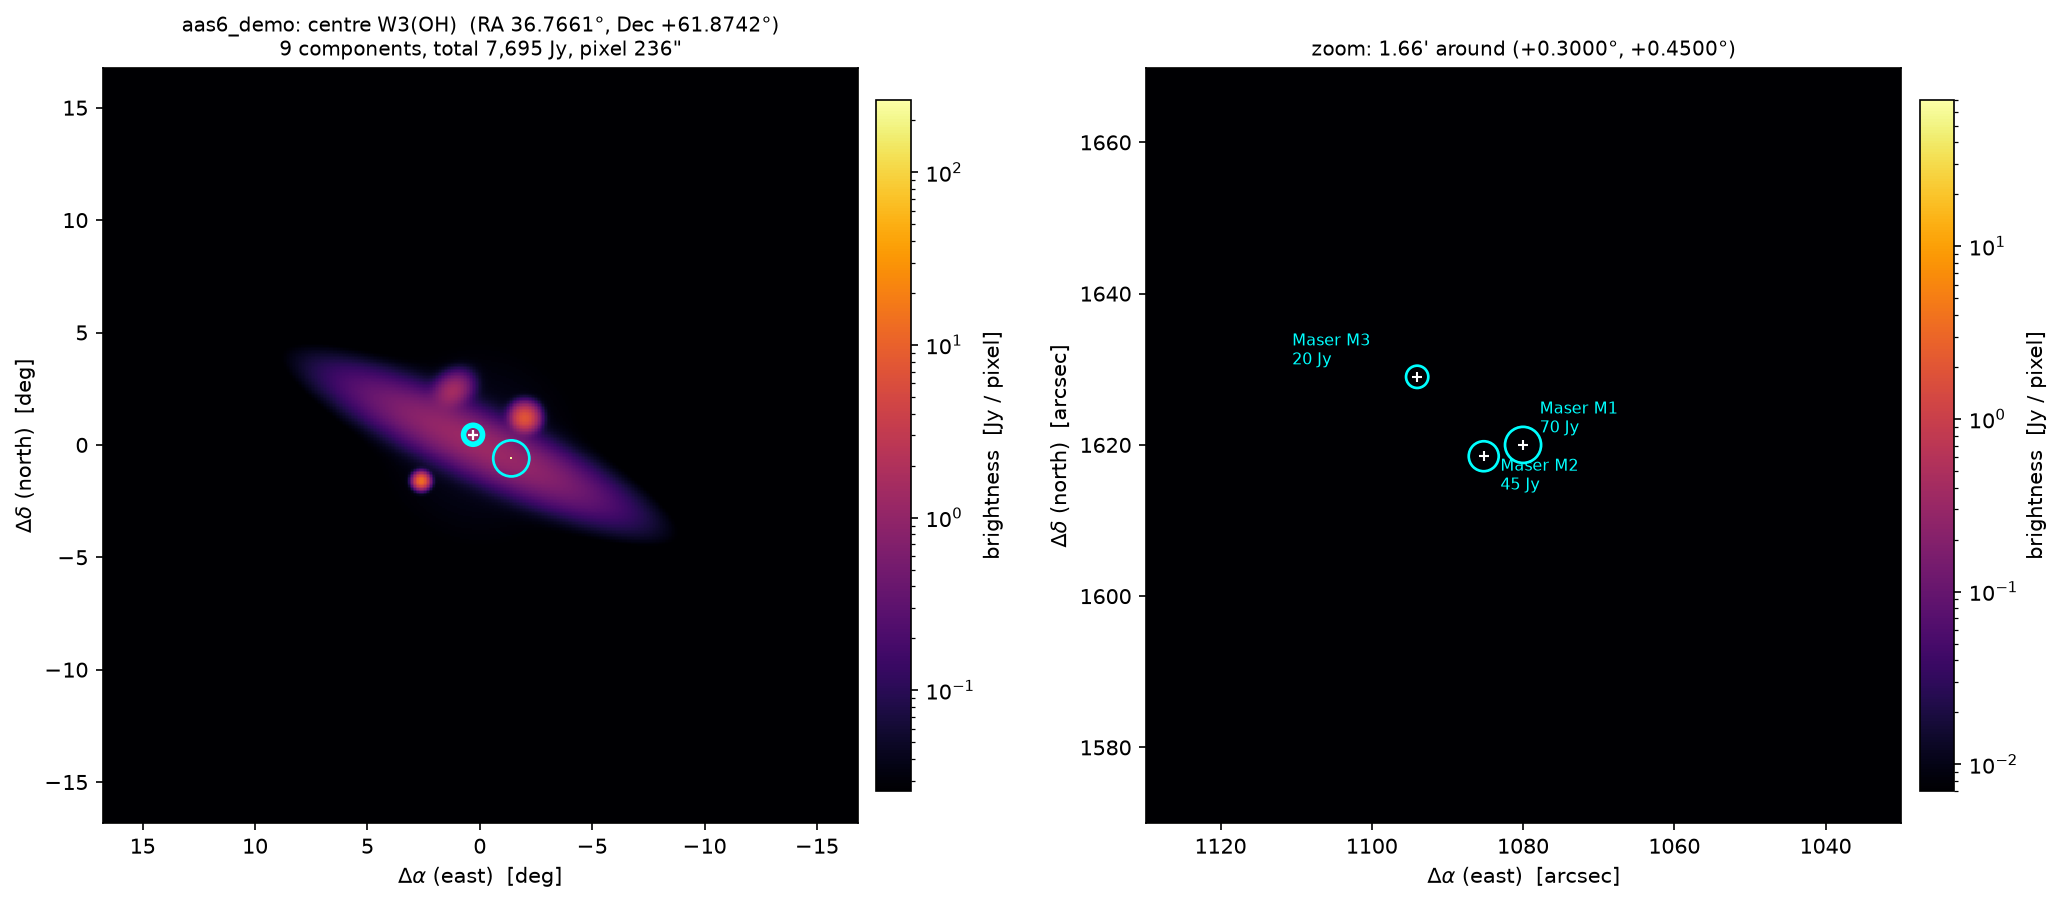
\includegraphics[width=\textwidth]{images/sky_demo_overview.png}
  \caption{Demo field \texttt{aas6\_demo.json}. Left: full field
           (logarithmic scale); right: zoom on the OH maser group, which
           is far below the pixel size of the full map.}
  \label{fig:sky-demo}
\end{figure}


	\chapter{Antennas}
	% docs/texte/20_core/antennas.tex -- chapter "Antennas" (Interferosim)
% Version: 0.3.0 (2026-10-12) -- implementation (interferosim 0.3.0), beam figure
%   0.2.0: antenna types and proposals
%   0.1.0: placeholder
% ================================================================
\index{antenna types}

All antennas derive from the abstract class \texttt{Antenna} (gain,
effective area, half-power beam width, beam pattern); the parameters are
read from \texttt{configs/antennas/} (chapter~\ref{ch:data-formats}).
The relations between gain, effective area and beam width are given in
chapter \enquote{Radio Astronomical Fundamentals}.

\section{Types of the first version}

\begin{center}
\begin{tabular}{@{}l>{\raggedright\arraybackslash}p{5.0cm}>{\raggedright\arraybackslash}p{5.6cm}@{}}
\toprule
Type & Parameters & Use in the project \\
\midrule
Horn & gain (15\,dBi) & two-horn test with the Sun (notebook~B) \\
Parabolic dish & diameter, aperture efficiency, beam factor
  (3\,m, 0.60, 1.20) & mapping, long baseline (notebook~A) \\
Yagi & number of elements, boom length, gain, design frequency;
  linear polarisation & low-cost station antenna \\
\bottomrule
\end{tabular}
\end{center}

\section{Implementation}
\label{sec:antennas-impl}

The module \texttt{interferosim.instrument.antennas} implements the three
types as subclasses of \texttt{Antenna} (Fig.~\ref{fig:uml-model}).
\texttt{Antenna.from\_toml()} reads a file of \texttt{configs/antennas/};
the key \texttt{type} selects the class. All methods take the frequency
as argument (default: HI line).
\begin{itemize}
  \item \texttt{gain\_dbi(f)}, \texttt{effective\_area(f)} with
        $A_\mathrm{eff} = G\lambda^2/4\pi$, \texttt{hpbw\_deg(f)},
        \texttt{beam(theta\_deg, f)} (normalised power pattern, 1 on the
        axis) and \texttt{jy\_to\_k(f)} $= A_\mathrm{eff}/2k$.
  \item \textbf{Horn} and \textbf{Yagi} are defined by their gain. The
        main lobe is a rotationally symmetric Gaussian with
        $\Omega_A = 1.133\,\theta_\mathrm{HPBW}^2 = 4\pi/G$, i.\,e.\
        \begin{equation}
          \theta_\mathrm{HPBW} = \sqrt{\frac{4\pi}{1.133\,G}}
        \end{equation}
        (notebook~B). The gain of the horn is frequency independent; with
        the optional key \texttt{design\_freq\_hz} it is treated as a fixed
        aperture ($G\propto f^2$). The Yagi gain is valid near its design
        frequency. The values in \texttt{yagi.toml} are typical example
        values (13 elements, boom $0.85\,\mathrm{m}\approx 4\lambda$,
        $15\,\mathrm{dBi}$) until the data of the actual antenna are known.
  \item The \textbf{parabolic dish} follows \texttt{aas6sim}:
        $A_\mathrm{eff} = \eta\,\pi D^2/4$,
        $\theta_\mathrm{HPBW} = k\lambda/D$ ($k = 1.2$ for tapered
        illumination). Its beam is the Airy pattern of the uniformly
        illuminated aperture with the same HPBW,
        $d_\mathrm{eff} = 1.02\,D/k$:
        \begin{equation}
          P(\theta) = \left[\frac{2J_1(x)}{x}\right]^2,\qquad
          x = \frac{\pi d_\mathrm{eff}\sin\theta}{\lambda}.
        \end{equation}
        \texttt{otf(u, f)} is the transfer function of the filled circular
        aperture with the cut-off $u_\mathrm{cut} = d_\mathrm{eff}/\lambda$
        (\texttt{u\_cut\_eff}); $u_\mathrm{max} = D/\lambda$ would make the
        beam too narrow.
\end{itemize}

\begin{center}
\begin{tabular}{@{}lrrrrr@{}}
\toprule
Antenna & $f$ [MHz] & $G$ [dBi] & $A_\mathrm{eff}$ [m$^2$] & HPBW [$^\circ$] & SEFD$^*$ [Jy] \\
\midrule
Dish 3\,m  & 1420.406 & 30.78 & 4.241 &  4.84 & 78\,129 \\
           & 1665.402 & 32.16 & 4.241 &  4.13 & 78\,129 \\
Horn 15\,dBi & 1420.406 & 15.00 & 0.112 & 33.93 & 2\,955\,887 \\
           & 1665.402 & 15.00 & 0.082 & 33.93 & 4\,063\,508 \\
Yagi 13 el. & 1420.406 & 15.00 & 0.112 & 33.93 & 2\,955\,887 \\
\bottomrule
\multicolumn{6}{@{}l}{\footnotesize $^*$ with the B210, $T_\mathrm{sys} = 120\,\mathrm{K}$ (chapter~\ref{ch:receiver})}
\end{tabular}
\end{center}

\begin{figure}[htbp]
  \centering
  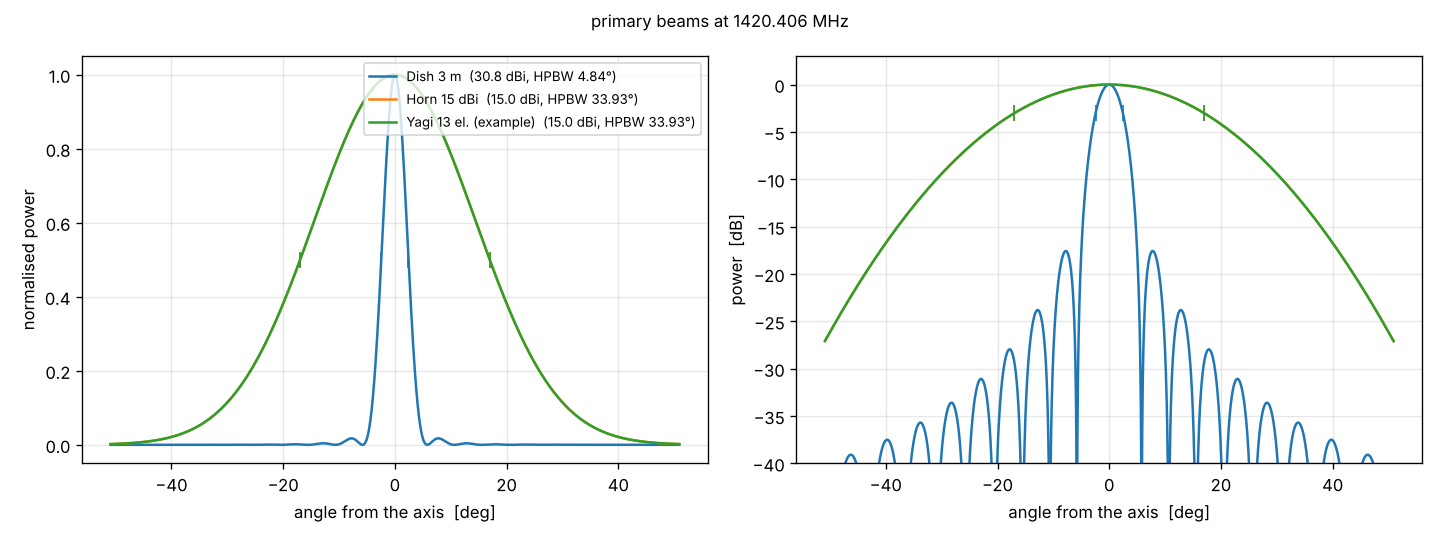
\includegraphics[width=\textwidth]{images/instrument_beams.png}
  \caption{Primary beams at $1420\,\mathrm{MHz}$ (\texttt{plot\_beams()}),
           linear and in dB; the bars mark the HPBW. Horn and Yagi
           coincide because both have $15\,\mathrm{dBi}$.}
  \label{fig:beams}
\end{figure}

\section{Proposals for further types}

\begin{center}
\begin{tabular}{@{}l>{\raggedright\arraybackslash}p{5.4cm}>{\raggedright\arraybackslash}p{5.2cm}@{}}
\toprule
Type & Properties & Why for Interferosim \\
\midrule
Axial-mode helix & circular polarisation, gain set by the number of
  turns, broader band than a Yagi & OH masers are often circularly
  polarised; Zeeman splitting (later extension) needs the circular
  components \\
Log-periodic dipole array (LPDA) & very broadband, moderate gain &
  one antenna for HI (1420\,MHz) and all four OH lines
  (1612--1720\,MHz) \\
Dipole (reference) & about 2.15\,dBi, very wide beam & reference
  antenna, Sun observations without tracking \\
Patch / patch array & flat, reproducible, gain grows with the number of
  patches & compact arrays of many elements for uv-coverage
  experiments \\
\bottomrule
\end{tabular}
\end{center}

Recommendation: helix and LPDA as the next two types -- the helix for the
polarisation of the OH lines, the LPDA for the frequency range of the
whole project. Further types need only a subclass of \texttt{Antenna}
and a configuration file.


	\chapter{Receiver}
	% docs/texte/20_core/receiver.tex -- chapter "Receiver" (Interferosim)
% Version: 0.1.0 (2026-10-12)
% ================================================================

Receiver model with system temperature and bandwidth; device profile
of the Ettus USRP B210 (two RX channels, common LO and clock) in
\texttt{configs/receivers/b210.toml}. \emph{Follows in phase~2.}


	\chapter{Observation}
	% docs/texte/20_core/observation.tex -- chapter "Observation" (Interferosim)
% Version: 0.2.0 (2026-10-31) -- section "Geometry" (module observation.geometry)
%   0.1.0 (2026-10-12): placeholder
% ================================================================
\label{ch:observation}

Hour angle and elevation (sidereal and solar day), uv-coverage with
Earth rotation synthesis, visibilities with noise, adding and
multiplying interferometer, fringe rate and delay.
The uv-coverage, the visibility simulation with noise and the transit
follow with version~0.5; the geometry needed by the signal simulation
(chapter~\ref{ch:signal}) is implemented since version~0.4.

\section{Geometry}
\index{geometric delay}\index{uvw}

The module \texttt{interferosim.observation.geometry} computes the source
direction in the earth-fixed frame (ECEF, chapter~\ref{ch:array}) from
right ascension $\alpha$, declination $\delta$ and the Greenwich hour angle
$H_G = \mathrm{GMST} - \alpha$ (or $H_G = H - \lambda$ from the local hour
angle $H$ at a site of longitude $\lambda$):
\begin{align}
  \hat s_0 &= (\cos\delta\cos H_G,\; -\cos\delta\sin H_G,\; \sin\delta),\\
  \hat e_E &= (\sin H_G,\; \cos H_G,\; 0),\qquad
  \hat e_N = (-\sin\delta\cos H_G,\; \sin\delta\sin H_G,\; \cos\delta),
\end{align}
$\hat s_0$ towards the phase centre, $\hat e_E$ and $\hat e_N$ east
(increasing $\alpha$) and north on the sky. A source at the offset $(l, m)$
lies in the direction $\hat s = \sqrt{1-l^2-m^2}\,\hat s_0 + l\,\hat e_E +
m\,\hat e_N$. GMST follows the IAU~1982 formula
$\mathrm{GMST} = 280.46061837^\circ + 360.98564736629^\circ\,(JD-2451545)$;
precession and nutation are neglected (AAS6 uses astropy; for the simulation
it suffices that simulator and correlator use the same model).

For a baseline $\vec B = \vec r_j - \vec r_i$ (station $i$ the reference):
\begin{align}
  \tau_g &= -\frac{\vec B\cdot\hat s}{c}
     && \texttt{geometric\_delay}\\
  (u, v, w) &= \frac{1}{\lambda}\,\bigl(\vec B\cdot\hat e_E,\;
               \vec B\cdot\hat e_N,\; \vec B\cdot\hat s_0\bigr)
     && \texttt{uvw}
\end{align}
$\tau_g > 0$ means the wavefront reaches station $j$ later. The delay rate
\texttt{delay\_rate} follows from the Earth's rotation
($\dot H_G = \omega_E$); for an east--west baseline it is
$\omega_E\,b\cos\delta\cos H/c$, maximal at transit. \texttt{elevation\_deg}
gives the elevation of a direction at a site.


	\chapter{Imaging}
	% docs/texte/20_core/imaging.tex -- chapter "Imaging" (Interferosim)
% Version: 0.1.0 (2026-10-12)
% ================================================================

Gridding, natural/uniform/Wiener weighting, dirty image and dirty beam
(PSF). \emph{Follows in phase~3.}


	\chapter{Deconvolution}
	% docs/texte/20_core/deconvolution.tex -- chapter "Deconvolution" (Interferosim)
% Version: 0.2.0 (2026-10-31) -- package interferosim.deconvolution (interferosim 0.8.0)
%   0.1.0 (2026-10-12): placeholder
% ================================================================
\label{ch:deconvolution-impl}
\index{deconvolution}\index{CLEAN}\index{clean beam}\index{Wiener filter}

H\"ogbom-CLEAN, Wiener filter, clean beam and restoration, comparison
metrics. Implemented in version~0.8.0 in the package
\texttt{interferosim.deconvolution} (classes as in the basic design,
Fig.~\ref{fig:uml-pipeline}); notebook \texttt{07\_deconvolution.ipynb}.
Origin: notebook~A of the teaching material (\texttt{hogbom\_fft}, clean beam
from the main lobe, comparison Wiener against CLEAN). Theory: chapter
\enquote{Deconvolution} in part \enquote{Theory}
(chapter~\ref{ch:deconvolution}).

\section{Implementation}

\begin{description}
  \item[\texttt{Deconvolver}] interface (strategy pattern):
        \texttt{deconvolve(dirty, beam, clean\_beam)} returns a
        \texttt{DeconvResult}; alias \texttt{run} as in the UML diagram.
  \item[\texttt{HogbomClean}] loop gain $g$, iteration limit, stop when the
        residual peak inside the window falls below
        $\max(\text{threshold}, \text{frac}\cdot\text{initial peak})$; CLEAN
        window as boolean mask or circles $(l, m, r)$; option
        \texttt{positive} (only positive peaks). The dirty beam of the
        \texttt{Imager} is periodic in the FFT grid, so the shift to the peak
        is a cyclic roll -- implemented as a slice of the twice-tiled beam
        without copying. The history stores the residual peak and the
        cumulative component flux per iteration.
  \item[\texttt{CleanBeam}] elliptical Gaussian (FWHM of major and minor
        axis, position angle east of north), fitted by least squares to
        $\ln B_D$ of the main-lobe pixels above 0.35; \texttt{kernel},
        \texttt{convolve} (model in Jy/pixel $\to$ image in Jy/beam, a point
        keeps its flux density as peak).
  \item[\texttt{DeconvResult}] model (Jy/pixel), residual and restored image
        $I_R = M * B_C + R$ (Jy/beam), clean beam, number of iterations,
        history; components brightest first, flux within a circle.
  \item[\texttt{WienerFilter}] $\mathcal W = \mathcal S^*/(|\mathcal S|^2 +
        \text{NSR}\cdot\max|\mathcal S|^2)$ with $\mathcal S$ = FFT of the
        dirty beam; \texttt{apply} optionally to the resolution of a target
        clean beam, \texttt{deconvolve} with residual
        $D - \hat I * B_D$.
  \item[\texttt{reference\_image}, \texttt{rms\_error}] the sky model on
        the pixel grid of an image, optionally attenuated per component by
        the primary beam (the apparent sky the visibilities measure) and
        convolved with the clean beam; rms difference within a circle.
\end{description}

\section{Results}

\paragraph*{OH masers with the project baseline.} The maser group of
chapter~\ref{ch:imaging} (natural weighting, grid $512\times0.25''$, loop
gain 0.1, threshold 0.45\,Jy/beam, positive components): CLEAN stops after
297 iterations, the residual has an rms of 0.16\,Jy/beam
(Fig.~\ref{fig:dec-masers}). The reference is the apparent sky: the masers
lie $0.54^\circ$ from the pointing centre, the primary beam of the 3\,m
dishes attenuates them to 0.96 of their flux density.

\begin{center}
\begin{tabular}{@{}lrrrrr@{}}
\toprule
Maser & true [Jy] & apparent & dirty & restored & CLEAN flux \\
\midrule
M1 & 70.0 & 67.0 & 62.0 & 65.4 & 65.3 \\
M2 & 45.0 & 43.0 & 33.7 & 41.0 & 41.2 \\
M3 & 20.0 & 19.1 & 25.3 & 17.9 & 18.0 \\
\midrule
\multicolumn{6}{@{}l}{rms error within $30''$: dirty 8.63, restored 0.19\,Jy/beam} \\
\bottomrule
\end{tabular}
\end{center}
The rms error drops by a factor of about 45. The remaining deficit of
1--2\,Jy per maser is the ambiguity of a single baseline: part of the flux
goes into components at sidelobe positions, where the fringe pattern of
the beam repeats (127 component pixels, 138\,Jy in total).

\begin{figure}[htbp]
  \centering
  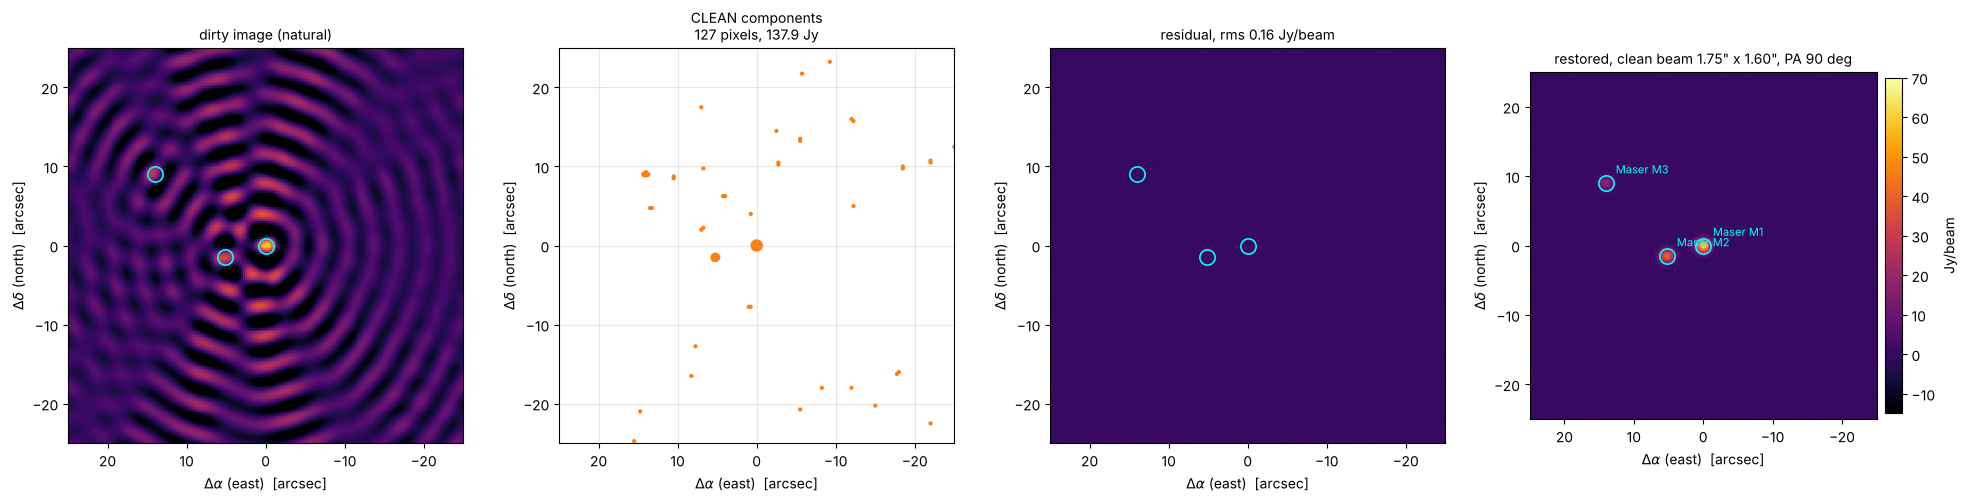
\includegraphics[width=\textwidth]{images/dec_clean_masers.png}
  \caption{CLEAN of the maser group with the project baseline: dirty image,
           CLEAN components (dot area $\propto$ flux), residual, restored
           image; circles: true positions.}
  \label{fig:dec-masers}
\end{figure}

\paragraph*{Convergence and loop gain.} The residual peak falls about
geometrically; $g = 0.05$, 0.1, 0.3 need 594, 297, 103 iterations with the
same rms error (0.19--0.20\,Jy/beam) (Fig.~\ref{fig:dec-gain}).

\begin{figure}[htbp]
  \centering
  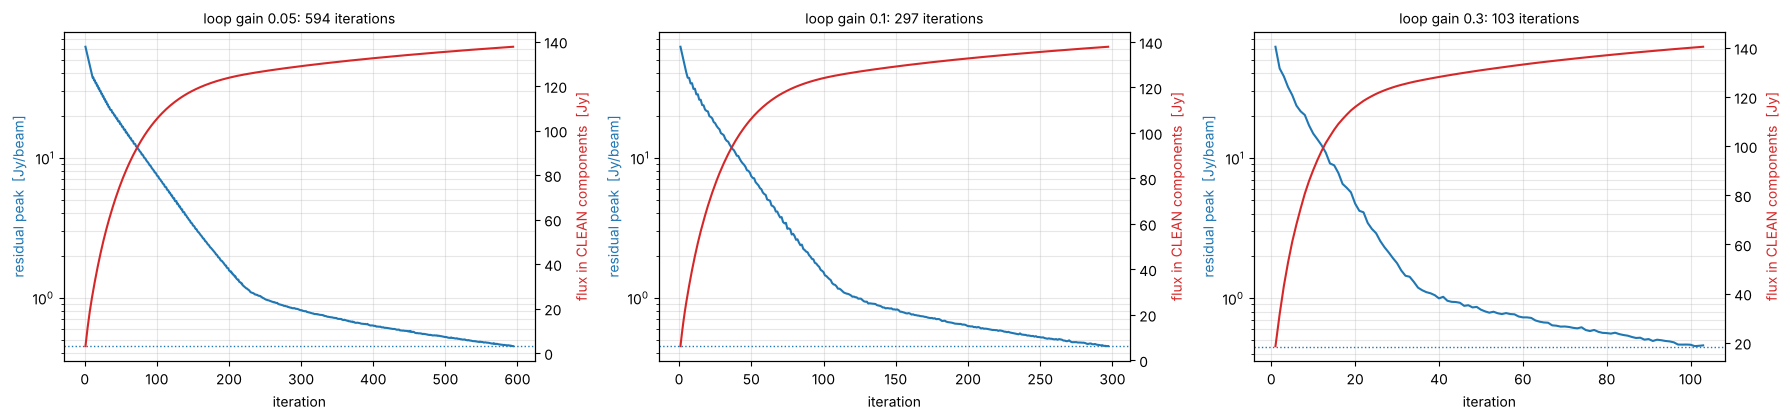
\includegraphics[width=\textwidth]{images/dec_clean_gain.png}
  \caption{Residual peak (blue, threshold dotted) and cumulative CLEAN flux
           (red) against the iteration for three loop gains.}
  \label{fig:dec-gain}
\end{figure}

\paragraph*{Wiener against CLEAN.} As in notebook~A, case~B
(Fig.~\ref{fig:dec-wiener}): only 292 of $512^2$ uv cells (0.11\,\%) are
measured. The Wiener weighting changes the beam only slightly (rms error
8.41\,Jy/beam), the Wiener filter keeps the measured cells and nothing else
-- its image is almost empty (1.3\,Jy/beam at M1). Its small rms error
(1.92\,Jy/beam) is misleading: an empty map is closer to a sparse truth
than a map full of sidelobes. Only the non-linear CLEAN recovers the masers
(0.19\,Jy/beam).

\begin{figure}[htbp]
  \centering
  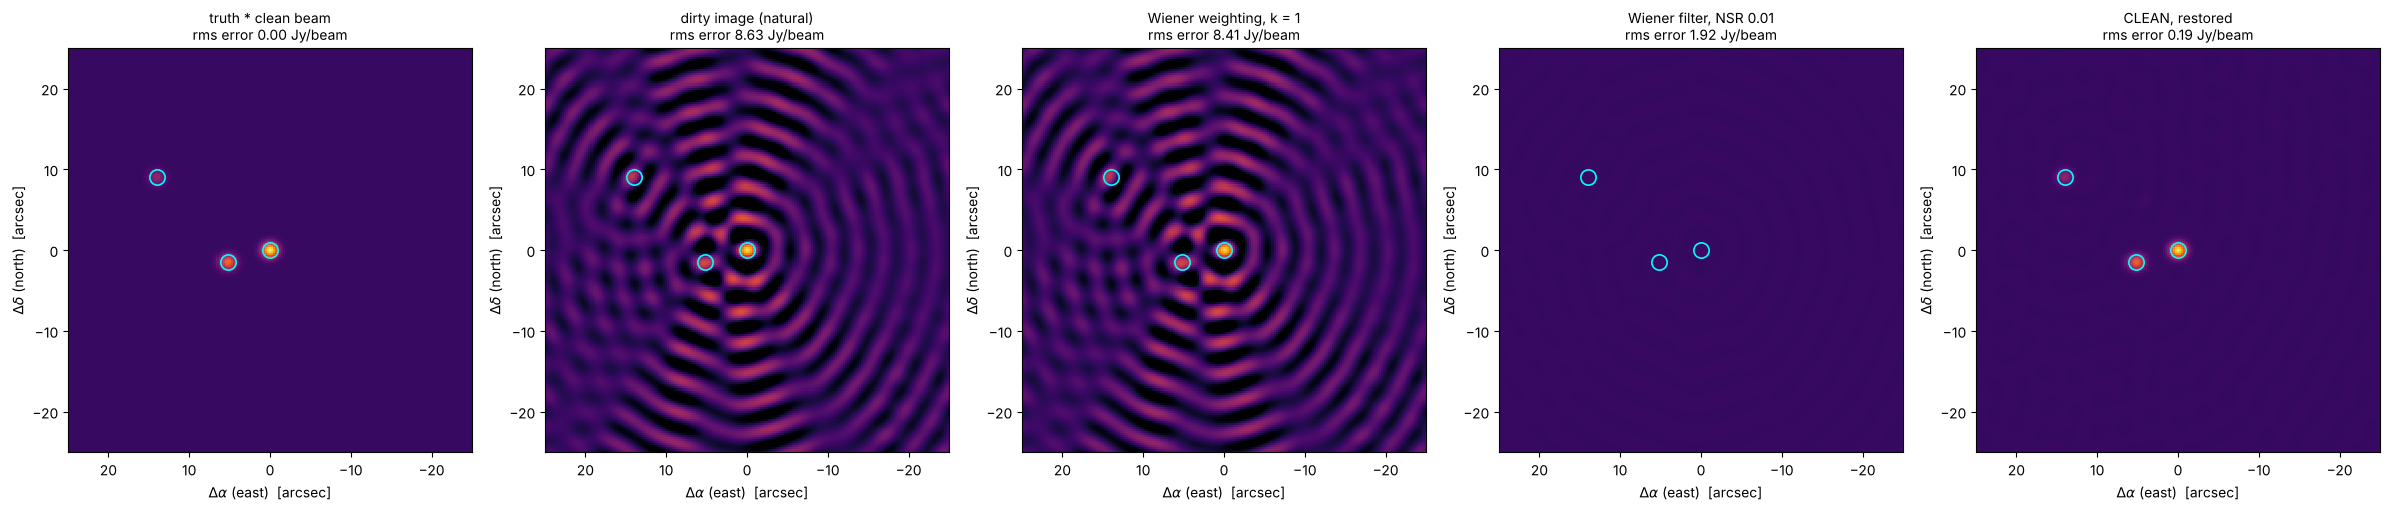
\includegraphics[width=\textwidth]{images/dec_wiener_clean.png}
  \caption{Truth (apparent sky $*$ clean beam), dirty image, Wiener weighting
           ($k=1$), Wiener filter (NSR 0.01, to clean-beam resolution) and
           restored CLEAN image.}
  \label{fig:dec-wiener}
\end{figure}

\paragraph*{More baselines.} With the hypothetical third station the CLEAN
flux densities of the three masers lie within 0.6\,Jy of the apparent ones
(single baseline: within 1.4\,Jy), with fewer spurious components
(Fig.~\ref{fig:dec-three}).

\begin{figure}[htbp]
  \centering
  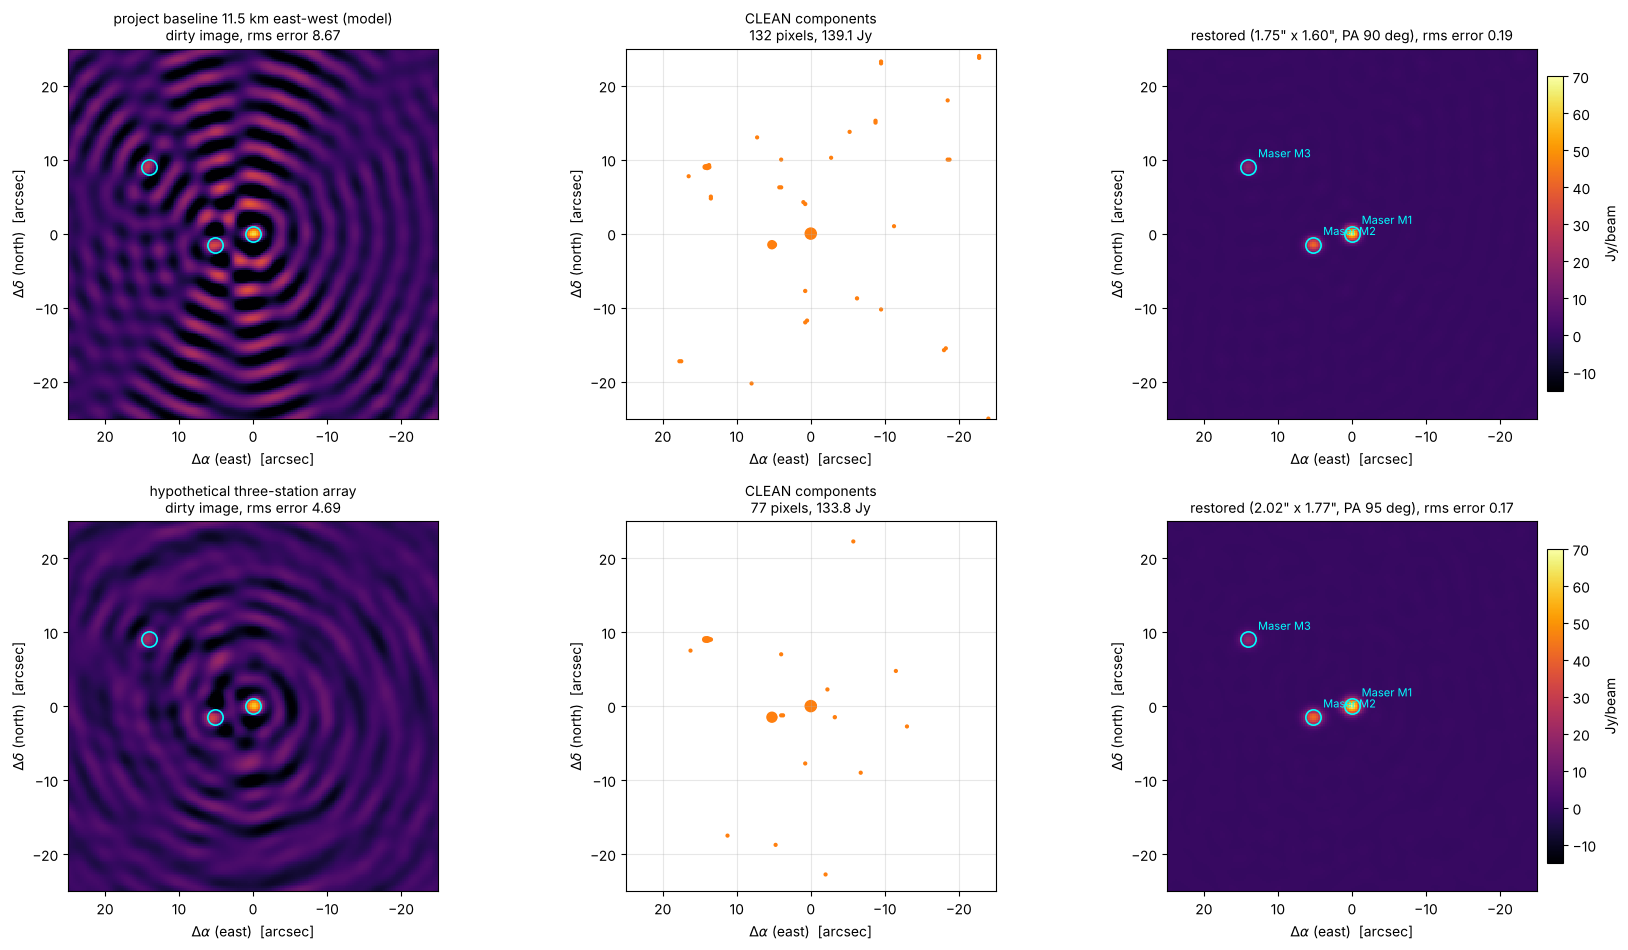
\includegraphics[width=\textwidth]{images/dec_clean_three.png}
  \caption{Project baseline alone (top) and with a hypothetical third station
           (bottom): dirty image, CLEAN components, restored image.}
  \label{fig:dec-three}
\end{figure}

\paragraph*{Limits: Cygnus~A.} CLEAN restores only what its components can
explain from the measured spatial frequencies. At 30--60\,k$\lambda$ the
lobes (${\approx}1400$\,Jy) are resolved out and even the hotspots (FWHM
$3''$) are partly resolved; CLEAN finds 9\,Jy (single baseline) or 49\,Jy
(three stations) of the 1556\,Jy, broken into hundreds of positive and
negative components along the fringes of the beam
(Fig.~\ref{fig:dec-cyga}). The restored image halves the rms error (1.8
$\to$ 0.9\,Jy/beam); with the single baseline its peak is even lower than
the dirty one, because the clean beam averages the alternating components.
Extended emission needs short baselines or single-dish data, and
deconvolution with other priors (multi-scale CLEAN, maximum entropy).

\begin{figure}[htbp]
  \centering
  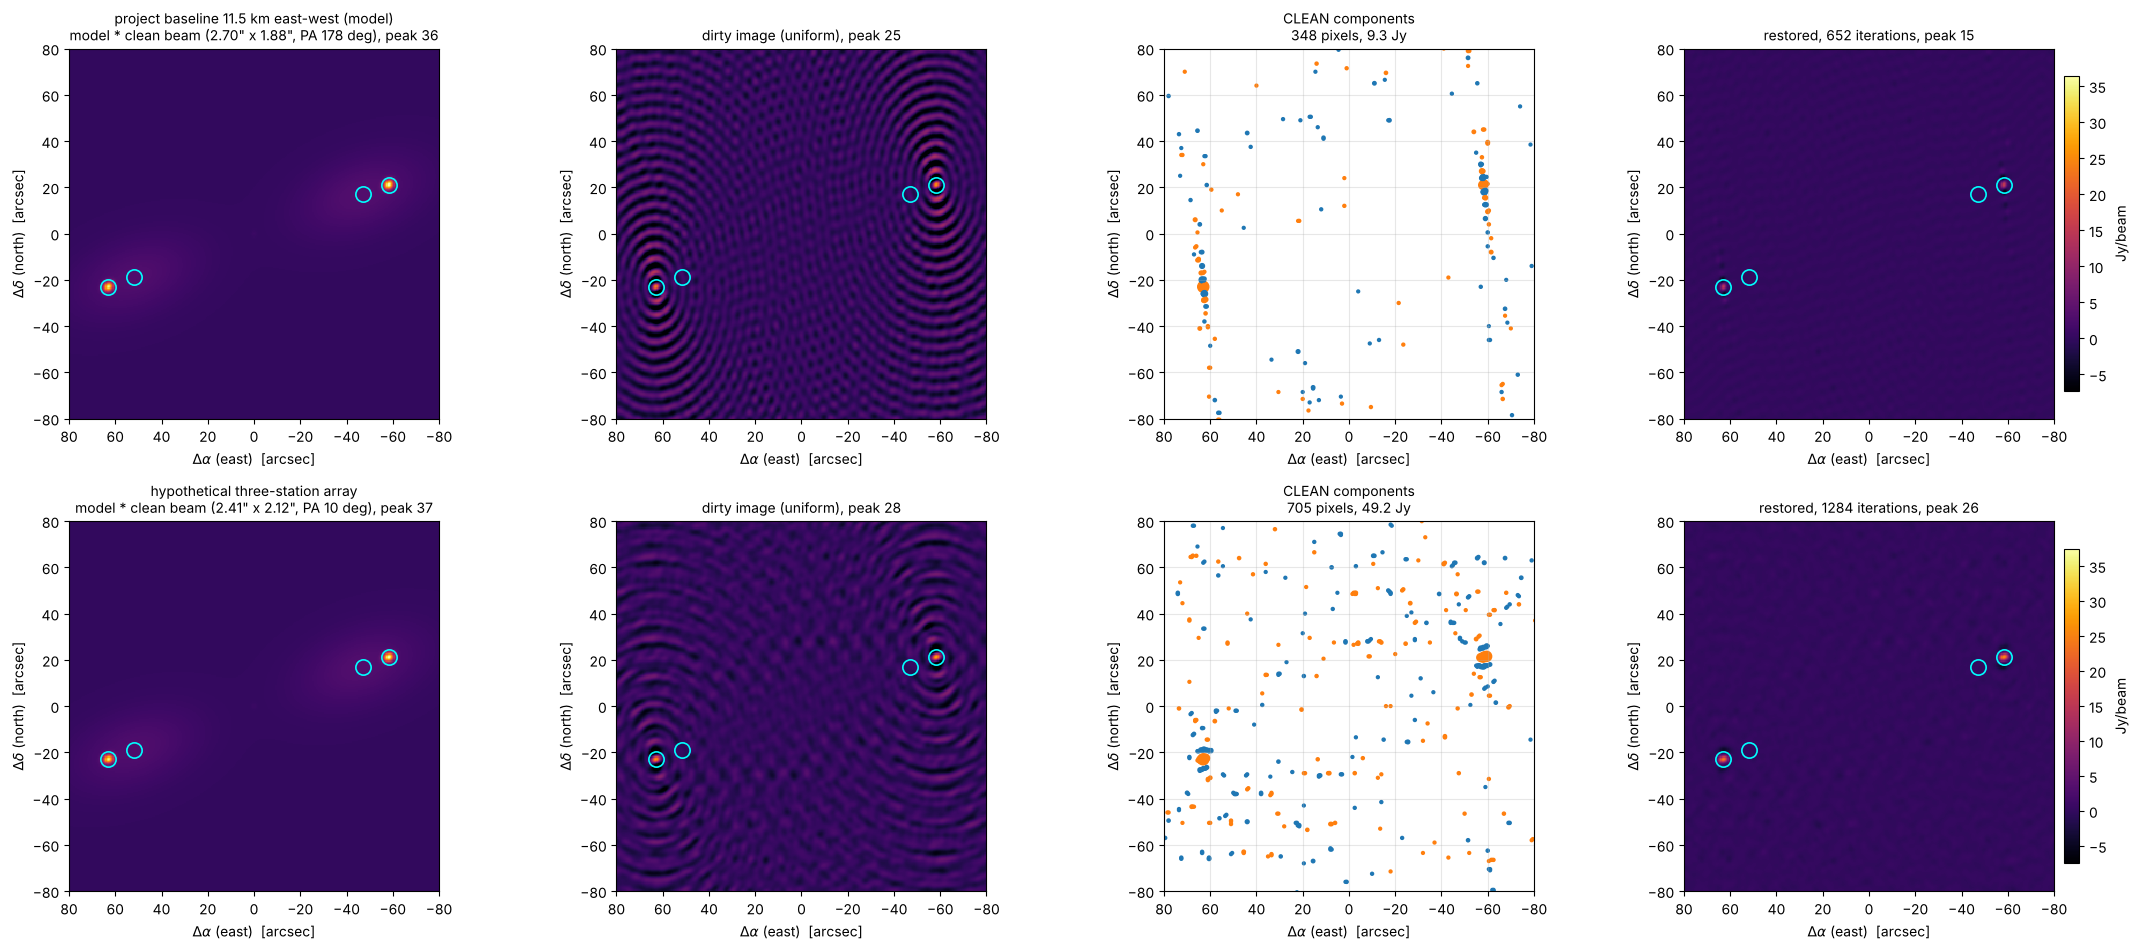
\includegraphics[width=\textwidth]{images/dec_clean_cyga.png}
  \caption{Cygnus~A at 1420\,MHz, project baseline (top) and three stations
           (bottom): apparent model $*$ clean beam, dirty image (uniform),
           CLEAN components (orange positive, blue negative), restored image;
           same colour scale per row.}
  \label{fig:dec-cyga}
\end{figure}


\part{Notebooks and Quality Assurance}

	\chapter{Interactive Notebooks}
	% docs/texte/30_notebooks/notebooks.tex -- chapter "Interactive Notebooks" (Interferosim)
% Version: 0.1.0 (2026-10-12)
% ================================================================

ipywidgets controls, interactive plots, one notebook per topic.
\emph{Follows in phase~4.}


	\chapter{Tests and Validation}
	% docs/texte/40_qa/tests.tex -- chapter "Tests and Validation" (Interferosim)
% Version: 0.1.0 (2026-10-12)
% ================================================================

Unit tests of the core package (pytest) and automated notebook runs
(nbval). \emph{Follows in phase~5.}

